\documentclass{article}
\usepackage[utf8]{inputenc}
\usepackage{CJKutf8}
\usepackage{graphicx}
\usepackage{subfig}
\usepackage{float}
\usepackage{subcaption}

\usepackage{tikz}
\usepackage{xcolor}

% Custom colors
\definecolor{process0}{RGB}{144,202,249}  % Light blue
\definecolor{process1}{RGB}{165,214,167}  % Light green
\definecolor{process2}{RGB}{255,204,128}  % Light orange
\definecolor{process3}{RGB}{206,147,216}  % Light purple
\definecolor{halocell}{RGB}{239,154,154}  % Light red

\usepackage{dirtree}

% Layout
\usepackage[left=1.5in, right=1.5in, top=1in, bottom=1in]{geometry}

% Images
\graphicspath{{./images/}}
\usepackage{wrapfig}
\usepackage{tabularx}
\usepackage{multirow}
\usepackage{totalcount}
\usepackage{caption}
\usepackage{subcaption}
\captionsetup{skip=0pt} 




% Math
\usepackage{amsmath,amssymb,amsthm,enumitem,bm}

\DeclareMathOperator{\sech}{sech}
\DeclareMathOperator{\csch}{csch}
\DeclareMathOperator{\arcsec}{arcsec}
\DeclareMathOperator{\arccot}{arcCot}
\DeclareMathOperator{\arccsc}{arcCsc}
\DeclareMathOperator{\arccosh}{arcCosh}
\DeclareMathOperator{\arcsinh}{arcsinh}
\DeclareMathOperator{\arctanh}{arctanh}
\DeclareMathOperator{\arcsech}{arcsech}
\DeclareMathOperator{\arccsch}{arcCsch}
\DeclareMathOperator{\arccoth}{arcCoth}

\usepackage{listings}
\usepackage{parskip}
\setlength{\parindent}{0pt}

\begin{document}
% Title
\begin{center}
    \huge\textbf{M2: Lora Finetuning}
\end{center}



\begin{center}
    \Large Xueqing Xu (xx823)
    
    Department of Physics, University of Cambridge
    
    April 7, 2025
\end{center}
Word Count: 2995
\subsection*{AI Declaration}
GitHub Copilot was used during development to assist with code completion, function documentation, and debugging. All AI-generated code underwent thorough review to ensure correctness, adherence to project requirements, and proper error handling. The core algorithms and methodological decisions remain my intellectual contribution, with Copilot serving only as a productivity tool for implementing standard techniques and reducing time spent on repetitive coding tasks.
\section*{Introduction}
We fine-tune the Qwen2.5-Instruct LLM for predator-prey population forecasting using Low-Rank Adaptation (LoRA). While LLMs can perform time series forecasting without explicit training\cite{gruver2023large}, we investigate how targeted fine-tuning enhances these capabilities under computational constraints.

LoRA injects trainable low-rank matrices into existing weights without modifying original parameters, dramatically reducing trainable parameter count. This parameter-efficient approach is ideal for large models under limited compute budgets.
\section*{Methodology}
\subsection*{Qwen2.5-Instruct model architecture}
The Qwen2.5-0.5B-Instruct model implements a decoder-only transformer architecture with 494 million parameters (Table \ref{tab:qwen25-overview}). With a hidden dimension of 896 across 24 transformer layers, the model balances depth and computational efficiency.

% Qwen2.5-0.5B-Instruct Model Overview Table
\begin{table}[ht]
\centering
\begin{tabular}{ll}
\hline
\textbf{Parameter} & \textbf{Value} \\
\hline
Model Type & Decoder-only Transformer \\
Parameters & 0.5 Billion \\
Hidden Size & 896 \\
Attention Heads & 14 \\
Head Dimension & 64 \\
Number of Layers & 24 \\
Intermediate Size (MLP) & 4864 \\
Vocabulary Size & 151,936 \\
\hline
\multicolumn{2}{l}{\textbf{Layer Structure (Repeated 24 times):}} \\
\hline
Pre-Attention & RMSNorm \\
Attention & Multi-head attention with RoPE \\
& \quad - Q, K, V projections \\
& \quad - Rotary Position Embeddings \\
Post-Attention & Residual connection \\
Pre-MLP & RMSNorm \\
MLP & Gate and Up projections \\
& SwiGLU activation \\
& Down projection \\
Post-MLP & Residual connection \\
\hline
\textbf{Final Output} & RMSNorm + Linear (LM head) \\
\hline
\end{tabular}
\caption{Qwen2.5-0.5B Model Architecture}
\label{tab:qwen25-overview} 
\end{table}


The model implements these components with a vocabulary of 151,936 tokens and tied word embeddings between input and output layers (Table \ref{tab:qwen25-vocab}). This architecture is particularly suitable for parameter-efficient fine-tuning methods like LoRA, as we can target high-leverage components (query and value projections) while keeping most parameters frozen.

% Qwen2.5-0.5B-Instruct Vocabulary Details Table
\begin{table}[H]
\centering
\begin{tabular}{@{}ll@{}}
\hline
\textbf{Property} & \textbf{Value} \\
\hline
Vocabulary Size & 151,936 tokens \\
BOS Token ID & 151,643 \\
EOS Token ID & 151,645 \\
Word Embeddings & Tied with output layer \\
\hline
\end{tabular}
\caption{Qwen2.5-0.5B-Instruct Vocabulary Details}
\label{tab:qwen25-vocab}
\end{table}

The model implements these components with a vocabulary of 151,936 tokens and tied word embeddings between input and output layers (Table \ref{tab:qwen25-vocab}). This architecture is particularly suitable for parameter-efficient fine-tuning methods like LoRA, as we can target high-leverage components (query and value projections) while keeping most parameters frozen.
\subsection*{Lora Finetuning}
Low-Rank Adaptation (LoRA) \cite{hu2022lora} represents a parameter-efficient fine-tuning approach that substantially reduces the number of trainable parameters while maintaining model performance. The key innovation lies in decomposing weight updates into low-rank matrices instead of fine-tuning the entire weight matrices.

\subsubsection*{Mathematical Formulation}

In standard fine-tuning of a pre-trained model, the weight matrix $W_0 \in \mathbb{R}^{d \times k}$ is updated to $W = W_0 + \Delta W$ during training. LoRA parameterizes the update $\Delta W$ using two low-rank matrices:

\begin{equation}
W = W_0 + \Delta W = W_0 + BA
\end{equation}

where $B \in \mathbb{R}^{d \times r}$ and $A \in \mathbb{R}^{r \times k}$ with rank $r \ll \min(d,k)$. During the forward pass, for input $x$, the output is computed as:


\begin{equation}
    h = W_0x + \Delta Wx = W_0x + BAx
    \end{equation}
    
    The weight update is typically scaled during training by $\alpha/r$, where $\alpha$ is a constant hyperparameter:
    
    \begin{equation}
    h = W_0x + \frac{\alpha}{r}BAx
    \end{equation}
    
    \subsubsection*{Application to Qwen2.5}
    
    For the Qwen2.5-0.5B-Instruct model, we apply LoRA specifically to the query and value projection matrices in the multi-head attention mechanism. These matrices are chosen because:
    
    \begin{itemize}
        \item Query projections ($W_q \in \mathbb{R}^{896 \times 896}$) directly influence the model's ability to focus on relevant context
        \item Value projections ($W_v \in \mathbb{R}^{896 \times 128}$) affect how the model represents information for aggregation
        \item Modifying these components provides substantial adaptation power while minimizing parameter count
    \end{itemize}
The LoRA matrices are injected into the model architecture, allowing for efficient adaptation without altering the original weights. The choice of low-rank matrices enables us to maintain a small number of trainable parameters while still achieving significant performance improvements.
    \subsubsection*{Training Dynamics}

During training, only the LoRA parameters ($A$ and $B$) are updated while $W_0$ remains frozen. This approach offers several advantages:

\begin{itemize}
    \item \textbf{Memory efficiency}: Only the gradients for LoRA parameters need to be stored
    \item \textbf{Composability}: Multiple task-specific LoRA modules can be trained and swapped without changing the base model
    \item \textbf{Preservation of general knowledge}: The original pre-trained weights remain intact
\end{itemize}

Additionally, we deviated from the standard LoRA approach by making the language model head trainable as well. This decision was motivated by the need for adaptation specifically at the vocabulary distribution level, which is crucial for accurate numerical predictions. The LM head contains $896 \times 151,936 = 136,134,656$ parameters, significantly increasing our trainable parameter count, but targeting this layer directly improves the model's ability to produce precise numerical outputs in text form.

The total trainable parameter count thus becomes:
\begin{align}
\text{LoRA parameters} + \text{LM head parameters} &= 344,064 + 136,134,656\\
&= 136,478,720
\end{align}

\subsection*{Predator-Prey Data}

\subsubsection*{Data Analysis}

Our exploratory analysis of the Lotka-Volterra dataset revealed important statistical properties across 1,000 trajectories. Each trajectory contained 100 time points with consistent sampling intervals. Data quality checks verified the absence of duplicates and negative values. 

Using K-means clustering on trajectory features (including period, amplitude, and phase relationships), we identified four distinct dynamic patterns in the dataset as displayed in Figure \ref{fig:clusters}:

\begin{itemize}
    \item \textbf{Classic oscillatory dynamics (14.6\%)}: Sustained oscillations with balanced prey-predator populations showing clear cyclic interactions.
    \item \textbf{Prey-dominant systems (69.3\%)}: Higher prey values with dampened predator oscillations, representing the majority of observed dynamics.
    \item \textbf{Equilibrium systems (14.9\%)}: Initially oscillating trajectories that quickly stabilize into steady states.
    \item \textbf{Predator collapse systems (1.2\%)}: Rare cases where predator populations collapse, allowing unconstrained prey growth.
    \end{itemize}

\begin{figure}[H]
    \centering
    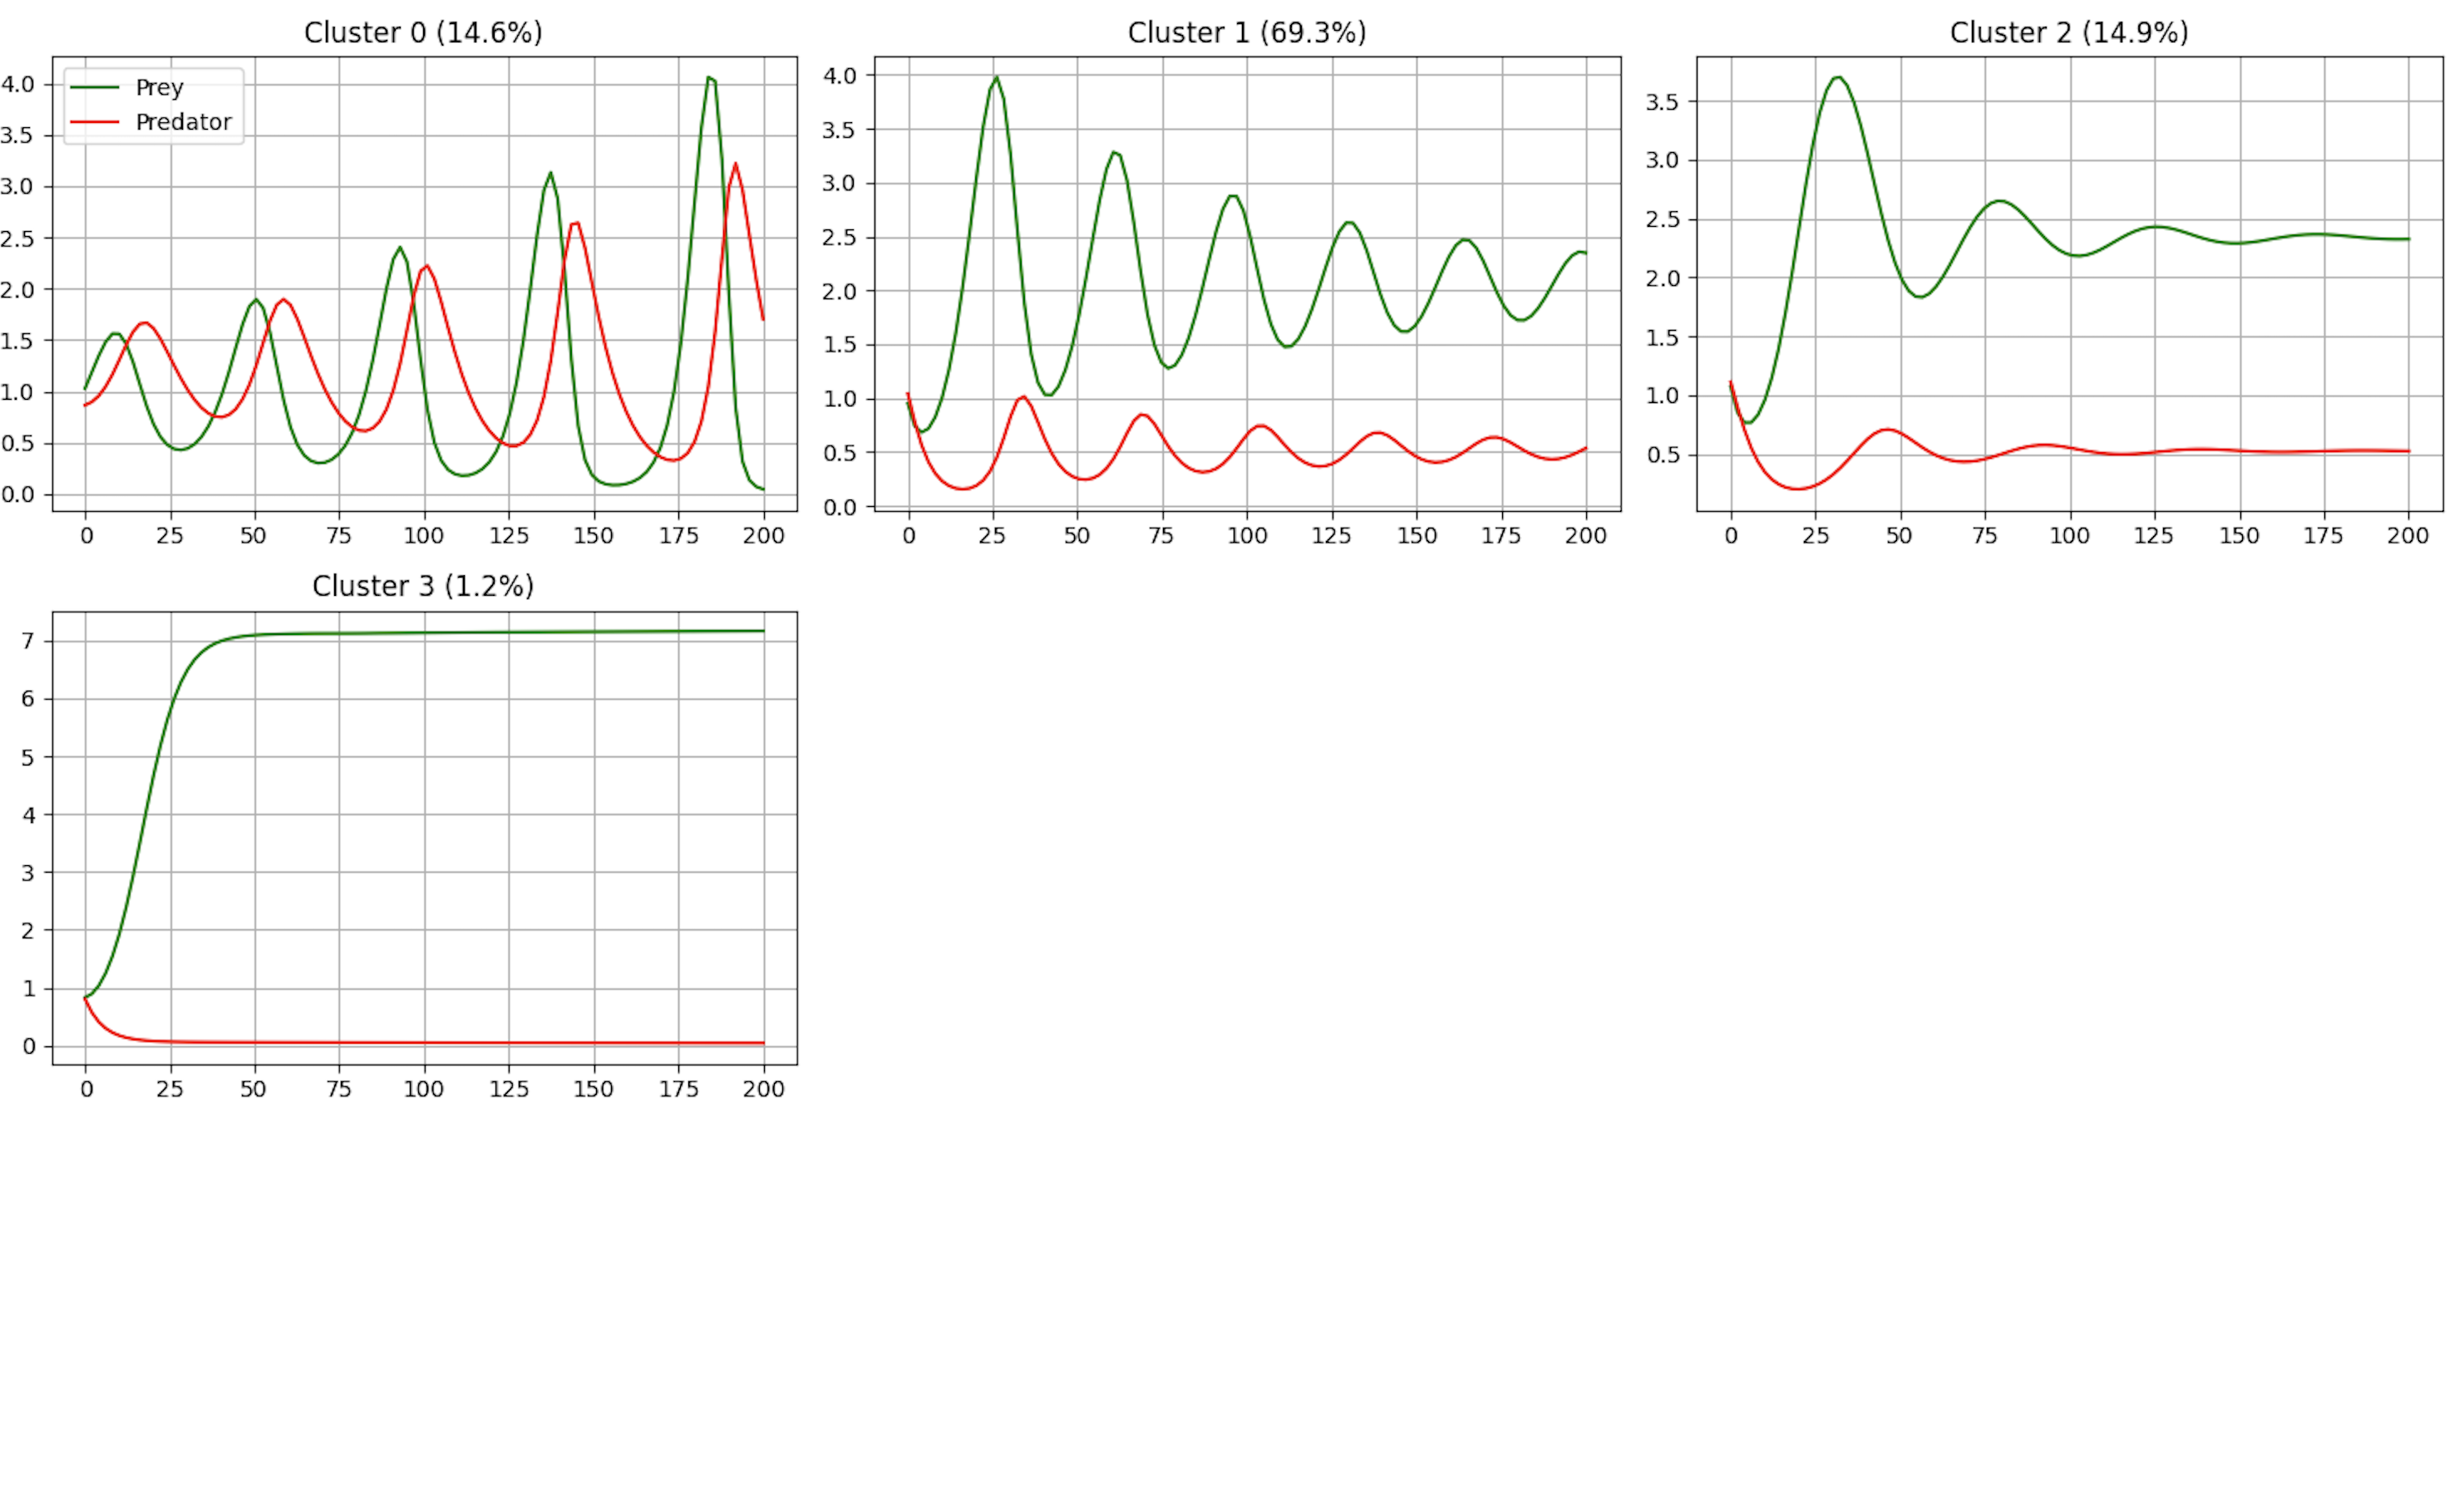
\includegraphics[width=0.8\textwidth]{cluster_representatives}
    \caption{\textbf{Cluster Analysis}. Four distinct clusters identified in the Lotka-Volterra dataset through K-means clustering}
    \label{fig:clusters}
\end{figure}

The clustering revealed that the majority of systems (69.3\%) fall into prey-dominant dynamics, suggesting parameter combinations that favor prey survival across much of the parameter space explored.

Figure \ref{fig:trajectories} showcases individual trajectories representing diverse dynamic behaviors within the dataset. These examples highlight the variability in amplitudes, frequencies, and phase relationships that our forecasting model must learn to predict accurately.

Through peak detection analysis, we calculated oscillation periods for both prey and predator populations, finding average periods of approximately 20-25 time units for prey and 20-30 time units for predators, as shown in Figure \ref{fig:periods}.

Further analysis of the phase relationships between prey and predator oscillations showed that predator peaks typically lag behind prey peaks by about 0.2 time units (20\% of the cycle period), as illustrated in Figure \ref{fig:periods}. This characteristic phase difference reflects the biological reality that predator populations grow in response to increasing prey availability, then decline as prey becomes scarce.

\begin{figure}[H]
    \centering
    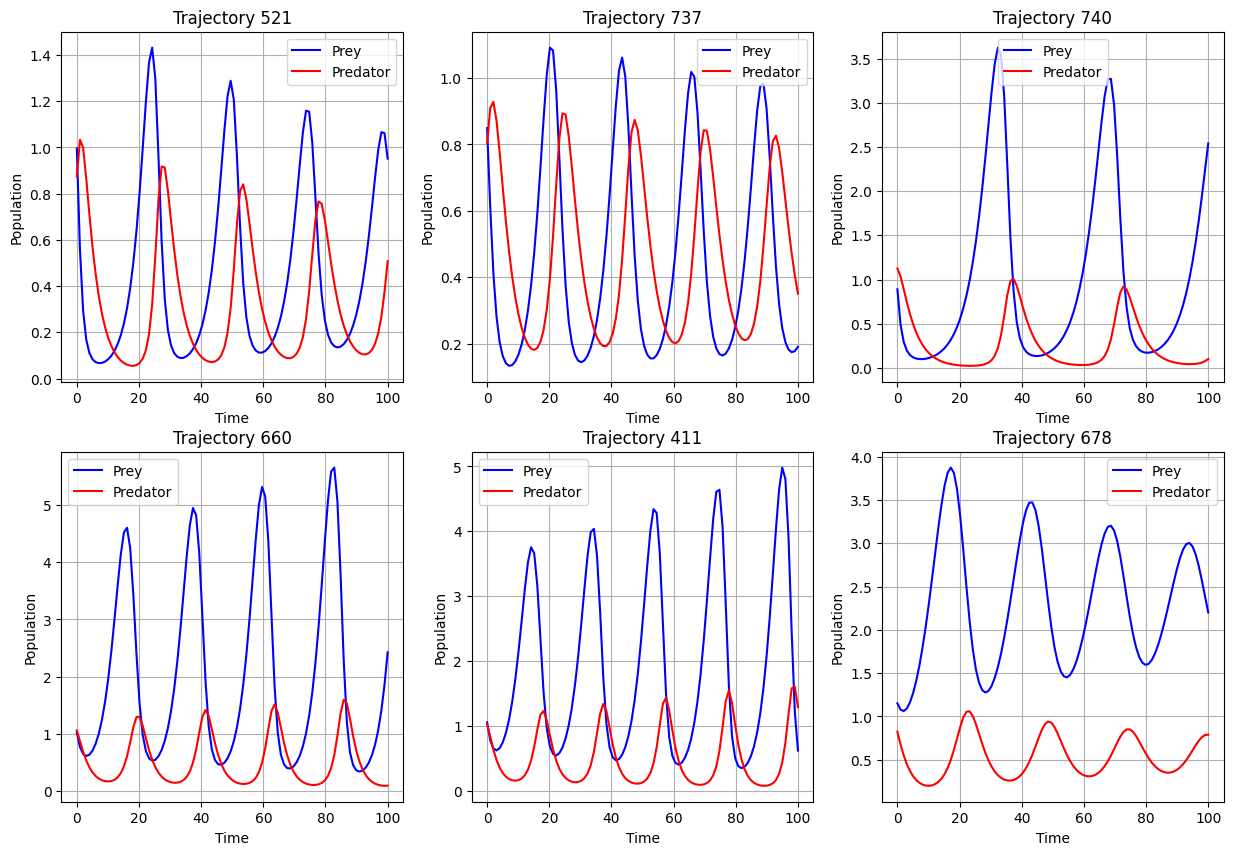
\includegraphics[width=0.8\textwidth]{sample}
    \caption{\textbf{Individual Trajectories}. Sample trajectories of prey and predator populations in the Lotka-Volterra dataset, illustrating the oscillatory dynamics characteristic of the model.}
    \label{fig:trajectories}
\end{figure}


\begin{figure} [H]
    \centering
    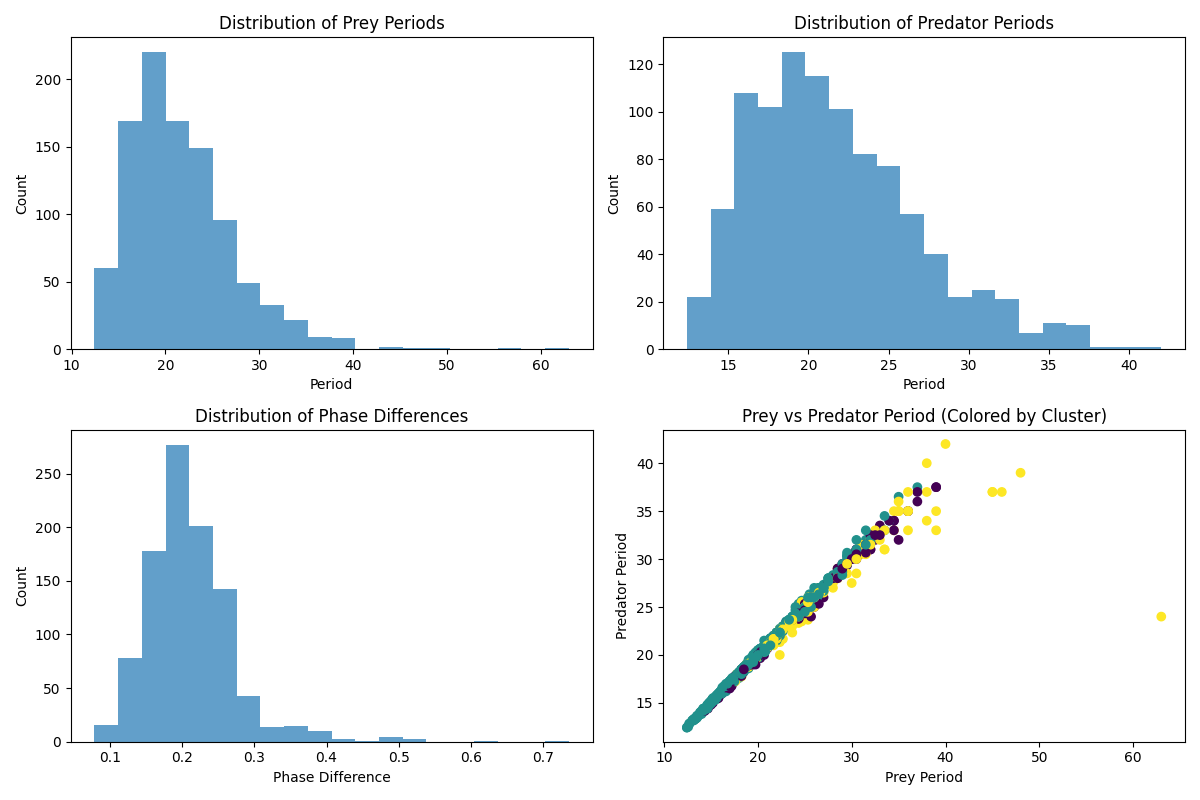
\includegraphics[width=0.8\textwidth]{period_distributions}
    \caption{\textbf{Statistical Distributions}. Distribution of oscillation periods for prey and predator populations in the Lotka-Volterra dataset, highlighting the variability in dynamics across different parameter regimes. }
    \label{fig:periods}
\end{figure}

Figure \ref{fig:average_trajectories} reveals typical system behavior with prey populations maintaining higher values (averaging $\approx$ 1.7 units) compared to predator populations (averaging $\approx$ 0.6 units) after initial transient dynamics.

\begin{figure} [H]
    \centering
    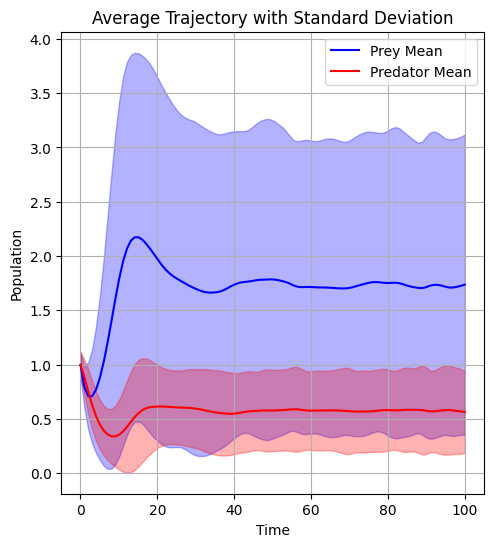
\includegraphics[width=0.5\textwidth]{overview_distribution}
    \caption{\textbf{Average Trajectories}. Average population trajectories with uncertainty: Mean prey (blue) and predator (red) population trajectories over time with shaded regions representing standard deviation.}
    \label{fig:average_trajectories}
\end{figure}

\begin{figure} [H]
    \centering
    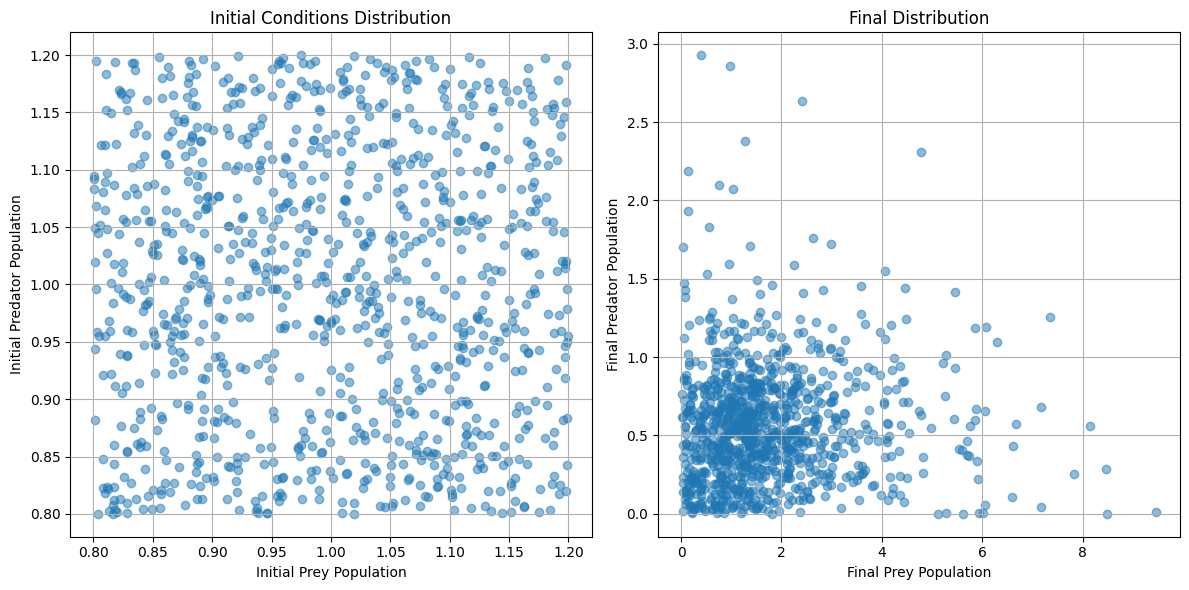
\includegraphics[width=0.8\textwidth]{initial_final_distribution}
    \caption{\textbf{Initial vs Final Distribution}. Comparison between initial conditions (left) and final states (right) of the predator-prey systems after simulation.}
    \label{fig:initial}
\end{figure}

Figure \ref{fig:initial} demonstrates the system's sensitivity to initial conditions. Despite narrowly ranged starting values (0.8-1.2), final states diverge dramatically—predator populations cluster at lower values (0.1-1.0) while prey populations spread widely (0-8). This characteristic divergence makes long-term forecasting challenging as small input variations amplify over time. For our 1,000-trajectory dataset, we used a simple random split (70/15/15\%), balancing practical constraints while acknowledging that larger future datasets would benefit from more sophisticated sampling approaches.
\subsubsection*{Future Improvements for Data Handling}
Future work with larger datasets should implement stratified sampling based on our identified clusters to maintain dynamic behavior distribution across all splits. This approach would ensure rare cases like "predator collapse" trajectories (1.2\%) are proportionally represented in training and evaluation sets, preventing the model from treating them as anomalies. Proper representation of all oscillation patterns and phase relationships is essential for comprehensive model training and evaluation.
\subsection*{LLMTIME Preprocessing Approach}

\subsubsection*{Text Representation Format}

We extended LLMTIME's \cite{gruver2023large} encoding approach for our multivariate data using commas to separate variables within timesteps and semicolons to separate sequential timesteps. Our implementation supports both 2-decimal (e.g., `2.46,10.25;1.92,7.68`) and 3-decimal precision formats, balancing accuracy with token efficiency.
\begin{itemize}
    \item Comma (“,") separates different variables at the same timestep
    \item Semicolon (“;") separates different timesteps in the sequence
\end{itemize}

Our implementation supports different numerical precision formats. Below are examples showing the same trajectory segment at 3-decimal and 2-decimal precision:

\begin{verbatim}
    2.458,10.249;1.916,7.677;1.503,5.985;...  # 3-decimal precision
    2.46,10.25;1.92,7.68;1.50,5.99;...        # 2-decimal precision
\end{verbatim}



\subsubsection*{Numerical Precision Considerations}

A critical aspect of our preprocessing is determining the appropriate precision for numerical values. We implemented and tested both 2 and 3 decimal place precision options:

\begin{equation}
x_{\text{text}} = \text{round}(x, d)
\end{equation}

where $d \in \{2,3\}$ is the decimal precision. Higher precision provides more accurate population values but increases token consumption and potentially makes patterns more difficult for the model to recognize. Our hyperparameter search included precision as an experimental variable to determine its impact on forecasting performance.

\subsubsection*{Data Scaling}

To ensure numerical stability and help the model work with a consistent range of values, we apply trajectory-specific scaling to the raw data before text conversion:

\begin{equation}
x_{\text{scaled}} = x \cdot \frac{\alpha}{P_{99}(x)}
\end{equation}

where $P_{99}(x)$ is the 99th percentile of the specific time series being processed and $\alpha=10.0$ is our target scale. This approach creates a unique scaling factor for each trajectory, ensuring that most values fall within the range $[0, \alpha]$ while preserving the relative dynamics and outliers within each sequence. 

\subsubsection*{Tokenization Effects}

The choice of text representation significantly impacts how the time series data is tokenized. For the Qwen2.5 tokenizer, numerical values are typically split into multiple tokens (e.g., 1.23 might tokenize as [1, ., 23]). Our analysis showed that each time step requires approximately 10-12 tokens, meaning that with a context length of 512 tokens, we can include roughly 40-50 time steps in the input context.

This tokenization behavior directly influenced our experimental design, particularly for evaluating optimal context length. By measuring the relationship between context length and prediction accuracy, we could determine how much historical information the model requires to make accurate forecasts.

\begin{table}[H]
\centering
\begin{tabular}{cp{3cm}cp{6cm}}
\hline
\textbf{Precision} & \textbf{Text} & \textbf{Token Count} & \textbf{Complete Token Sequence} \\
\hline
\multirow{2}{*}{2 decimal} & 10.02,10.03;7.81,7.51 & 21 & [16, 15, 13, 15, 17, 11, 16, 15, 13, 15, 18, 26, 22, 13, 23, 16, 11, 22, 13, 20, 16] \\
\cline{2-4}
    & 9.01,10.02;10.01,8.19 & 21 & [24, 13, 15, 16, 11, 16, 15, 13, 15, 17, 26, 16, 15, 13, 15, 16, 11, 23, 13, 16, 24] \\
\hline
\multirow{2}{*}{3 decimal} & 9.015,10.018;10.010,8.189 & 25 & [24, 13, 15, 16, 20, 11, 16, 15, 13, 15, 16, 23, 26, 16, 15, 13, 15, 16, 15, 11, 23, 13, 16, 23, 24] \\
\cline{2-4}
    & 10.022,10.025;7.813,7.510 & 25 & [16, 15, 13, 15, 17, 17, 11, 16, 15, 13, 15, 17, 20, 26, 22, 13, 23, 16, 18, 11, 22, 13, 20, 16, 15] \\
\hline
\end{tabular}
\caption{Complete tokenization comparison between 2-decimal and 3-decimal precision formats for predator-prey data.}
\label{tab:precision_comparison}
\end{table}
\subsubsection*{Text-to-Numeric Conversion}

To convert model outputs back to numerical values, we implemented a parsing function that splits text by delimiters (commas and semicolons) and reverses scaling. Our error-handling system uses regex pattern matching to process inconsistently formatted values, handles missing data, enforces non-negativity constraints for population data, and ensures dimensional consistency. These safeguards guarantee that our evaluation metrics reflect actual forecasting errors rather than parsing artifacts.
\subsubsection*{Training Data Processing}

For model training, we processed the data as follows:
\begin{enumerate}
    \item Split the 1,000 trajectories into train (70\%), validation (15\%), and test (15\%) sets
    \item Convert numerical trajectories to text format with specified precision and scaling
    \item For training data, create overlapping chunks with sequence length 512 and stride 256
    \item For validation, create non-overlapping chunks to prevent information leakage
    \item For testing, maintain complete trajectories without chunking
\end{enumerate}

\subsection*{FLOPs Calculation}

We implemented detailed FLOP tracking to quantify computational costs across our experiments. Our calculations account for all transformer operations (embedding, attention with LoRA modifications, feed-forward networks, normalization layers, and language model head). 

With batch size $B=4$, sequence length $S=512$, and LoRA rank $r=8$, we determined that each training step required approximately $5.94 \times 10^{12}$ FLOPs (including backward pass). We maintained our total experimental budget of $10^{17}$ FLOPs, allocating 50\% to hyperparameter search, 15\% to context length evaluation, and 35\% to final model training. Complete equation derivations and detailed FLOP accounting are provided in the Appendix.
\section*{Implementation}

\subsection*{Hardware}
Experiments were conducted on NVIDIA A100 GPUs (40GB RAM) with model inference performed on M1 Pro (16GB RAM), using automatic device selection (CUDA/MPS/CPU) based on availability.
\subsection*{Model training setup}
\subsubsection*{Optimization Approach}

We employed the AdamW optimizer with weight decay of 0.01, which helps mitigate overfitting during fine-tuning. Gradient clipping at 1.0 was applied to prevent exploding gradients, which is particularly important when fine-tuning large language models. For each training step, we logged both pre-clipping and post-clipping gradient norms, maintaining a ratio typically between 0.8-1.0, indicating stable training dynamics.

We utilized the OneCycleLR scheduler which provides effective learning rate management. This approach allows the model to initially adapt quickly and then gradually refine its parameters.

\subsubsection*{Validation Setup}
During training, validation runs occurred every 500 steps using 20 randomly sampled trajectories to calculate MAE and MSE metrics for 10-step-ahead predictions. We implemented checkpointing to save the best-performing model based on these metrics to prevent overfitting.

\subsection*{Evaluation Setup}
Our evaluation pipeline implements a rigorous approach for assessing forecasting accuracy:
\subsubsection*{Forecasting Process}

For each test trajectory, we:
\begin{enumerate}
    \item Provide the first 50 timesteps as context
    \item Generate the next 50 timesteps autoregressively
    \item Apply post-processing to ensure valid numerical formatting
    \item Compare predictions against ground truth values
\end{enumerate}

To ensure robustness, we implemented pattern-matching techniques that correct common errors in the model's text generation, such as inconsistent decimal places or missing delimiters.

\subsubsection*{Evaluation Metrics}

We calculated the following metrics to assess model performance:
\begin{itemize}
    \item \textbf{Error metrics}: MAE (primary), MSE (penalizes larger errors), and population-specific variants for prey and predator separately
    \item \textbf{Success rate}: Percentage of trajectories yielding valid numerical predictions
\end{itemize}

All evaluations used 150 test trajectories with performance tracked across all timesteps.

\subsubsection*{Generation Settings}

For model generation, we followed the same approach as the original LLMTIME paper \cite{gruver2023large}, using stochastic sampling with temperature 0.9 and top-p 0.9:

\begin{verbatim}
output = model.generate(
    inputs["input_ids"],
    max_new_tokens=max_tokens,
    temperature=0.9,
    top_p=0.9,
    do_sample=True,
    renormalize_logits=True
)
\end{verbatim}

This configuration provides a balance between diversity and coherence in generated sequences, which is particularly important for producing accurate numerical forecasts while maintaining the ability to capture the range of possible system behaviors.
\section*{LoRA Experiments}
\subsection*{Hyperparameter search experiment}
To optimize our LoRA fine-tuning approach, we conducted a comprehensive grid search over key hyperparameters, evaluating their impact on forecasting accuracy while respecting our computational budget constraints.

\subsubsection*{Experimental Configuration}
Our hyperparameter search explored 18 different configurations across three dimensions:
\begin{itemize}
    \item Learning rates: 1e-5, 5e-5, 1e-4
    \item LoRA ranks: 2, 4, 8
    \item Precision values: 2, 3 decimal places
\end{itemize}

For each configuration, we maintained consistent values for:
\begin{itemize}
    \item Context length: 128 tokens (optimized in a separate experiment)
    \item LoRA dropout: 0.05
    \item LoRA $\alpha$: 2 $\times$ rank value
\end{itemize}
\subsubsection*{Results and Analysis}
\begin{figure}[h]
    \centering
    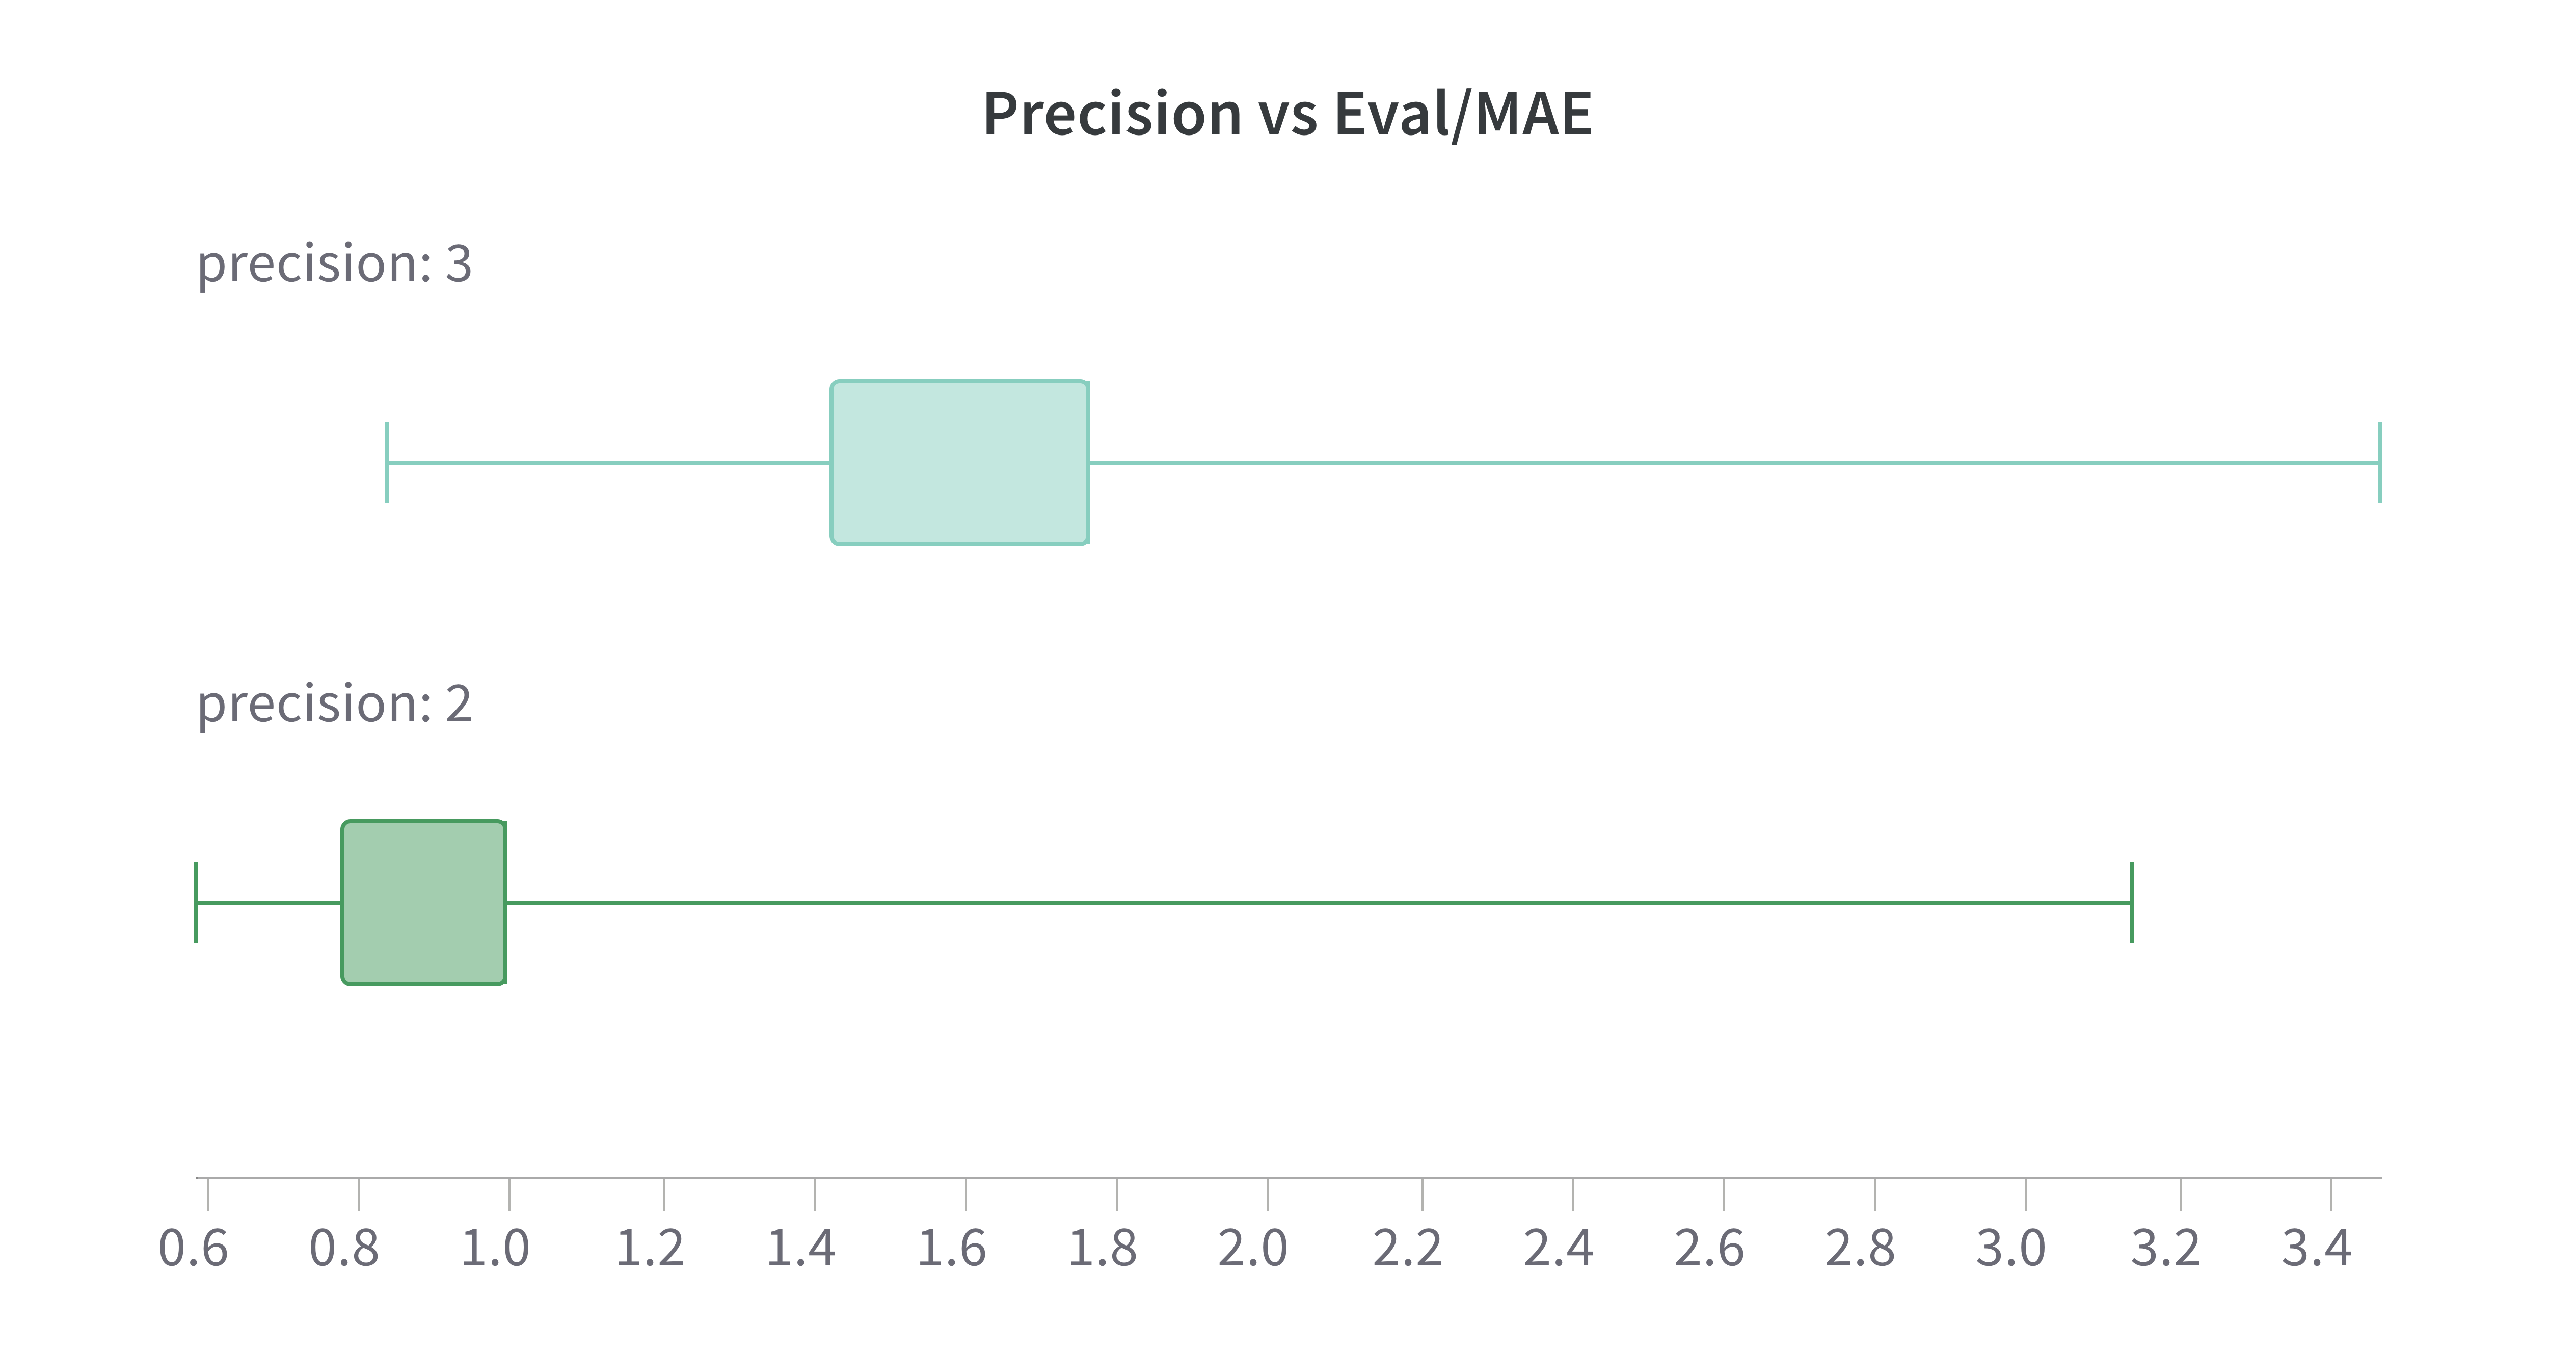
\includegraphics[width=0.48\textwidth]{precision}
    \caption{\textbf{Effect of Precision on Model Performance}. Validation MAE for different precision values across hyperparameter configurations.}
    \label{fig:hp_precision}
\end{figure}

\begin{figure}[h]
    \centering
    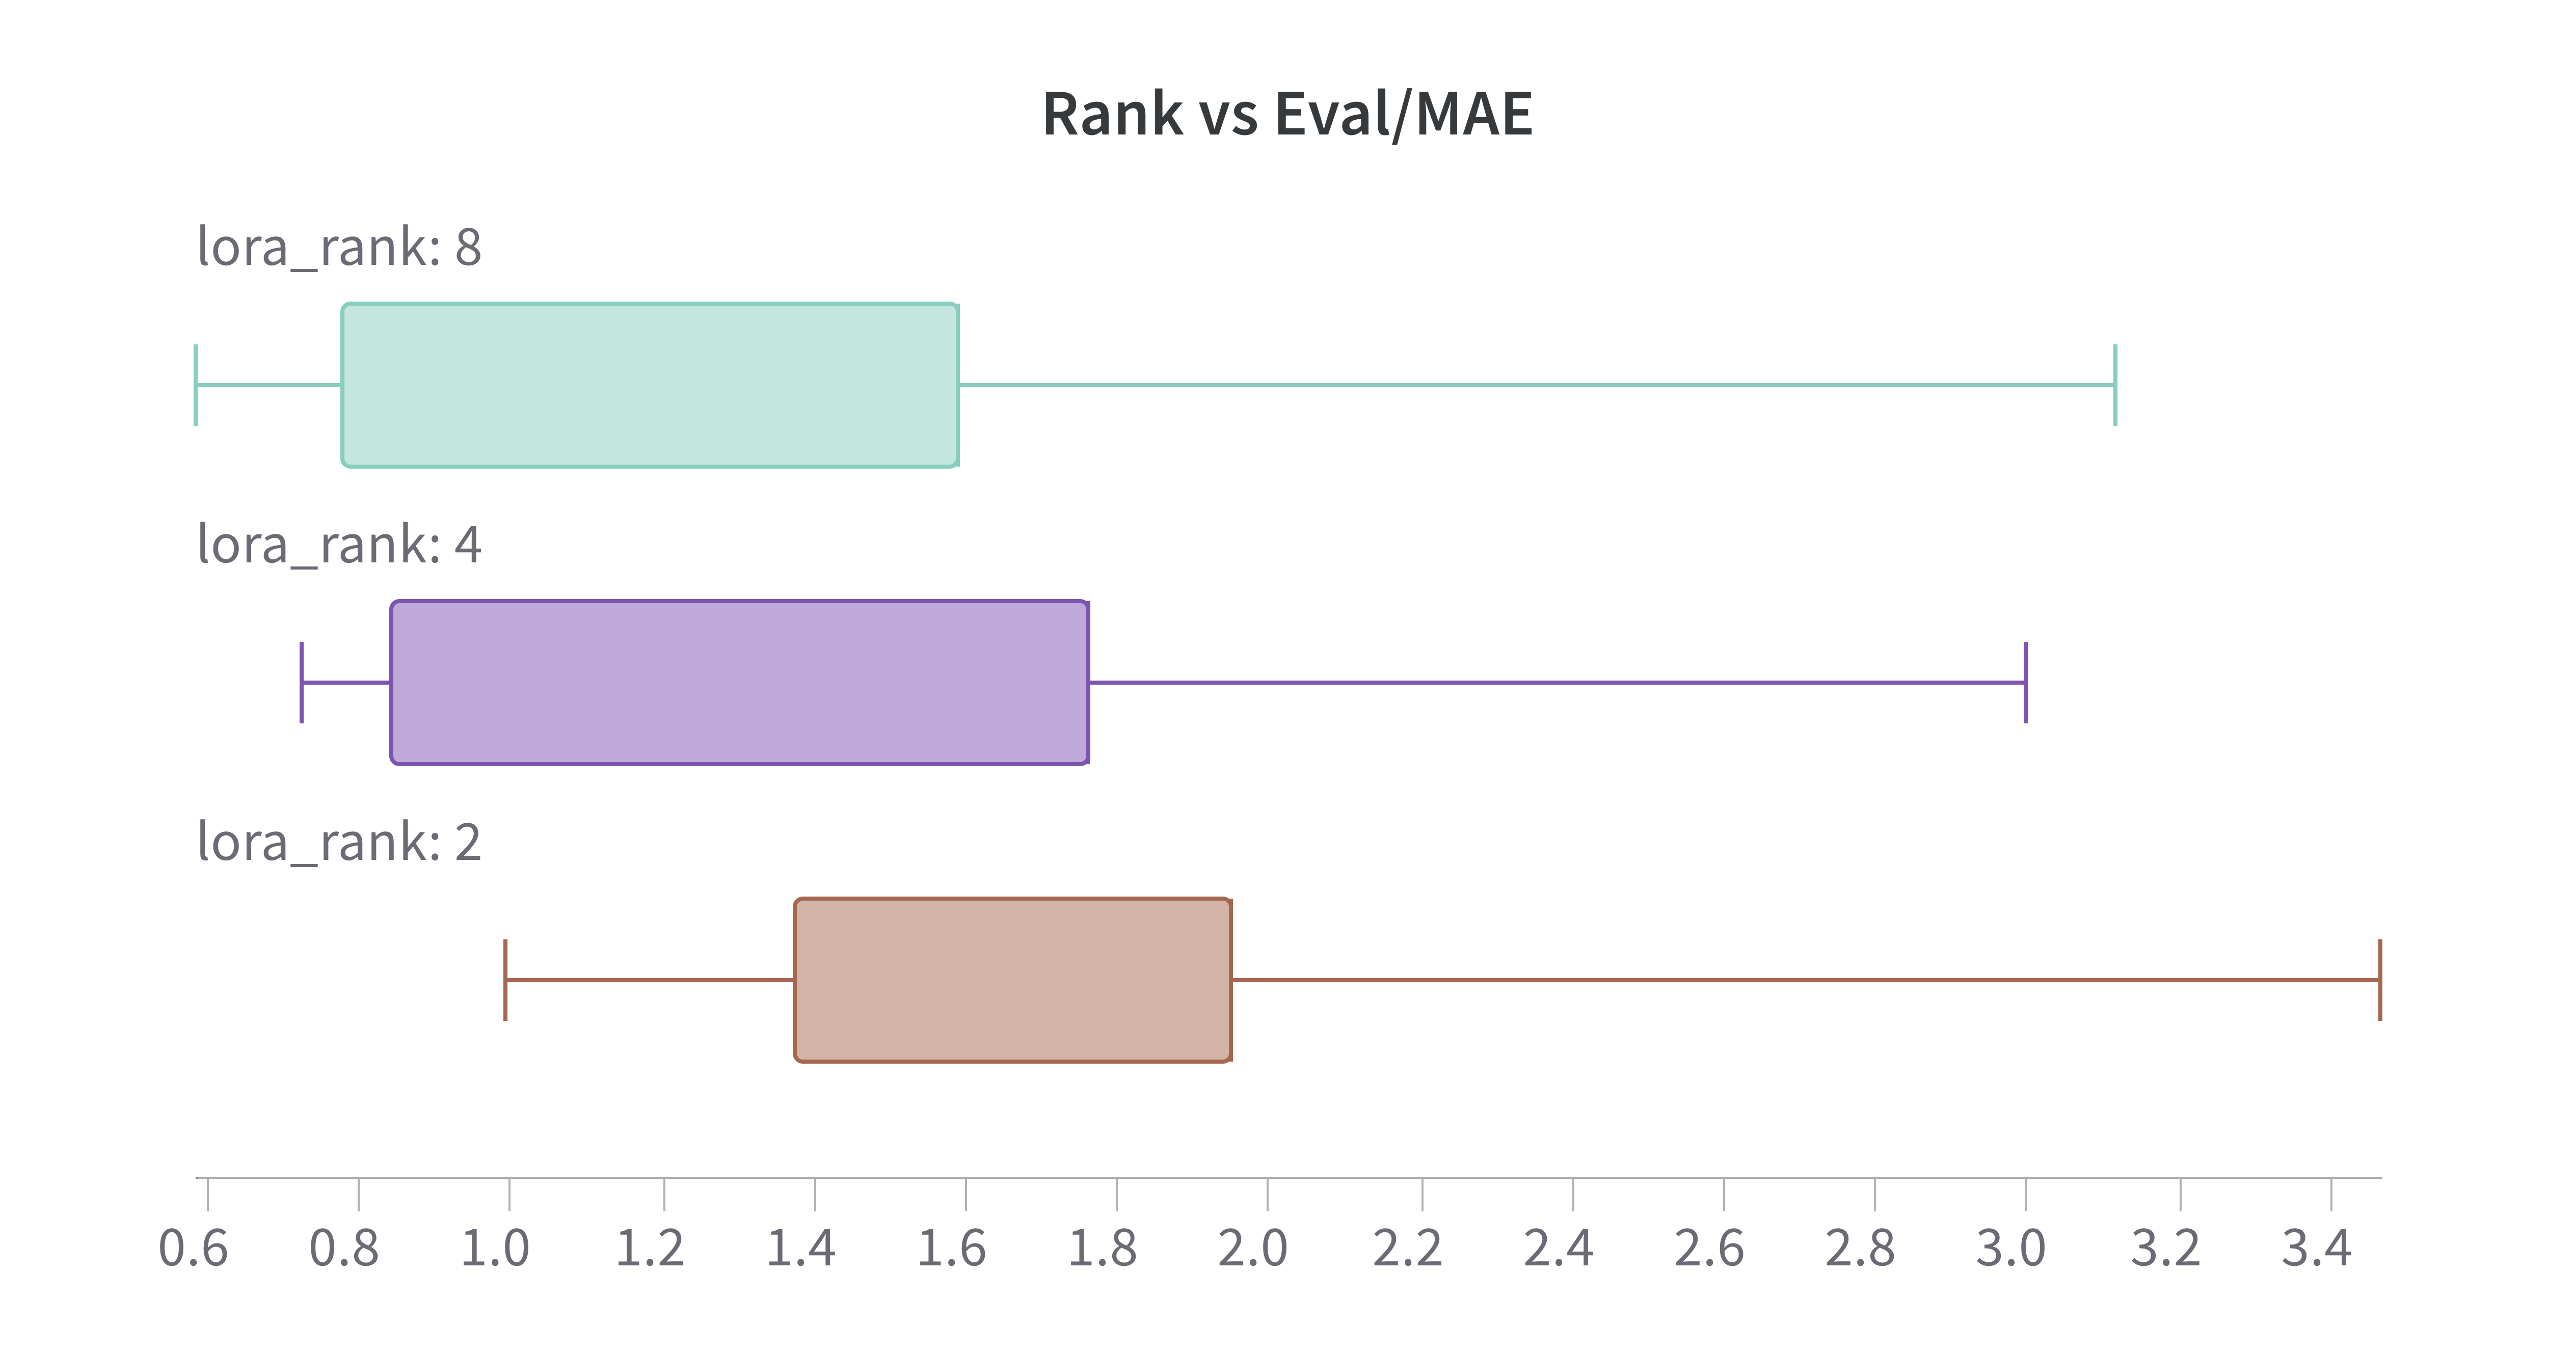
\includegraphics[width=0.48\textwidth]{rank}
    \caption{\textbf{Effect of LoRA Rank on Model Performance}. Validation MAE for different rank values (2, 4, 8) showing improved performance with higher rank.}
    \label{fig:hp_rank}
\end{figure}

\begin{figure}[h]
    \centering
    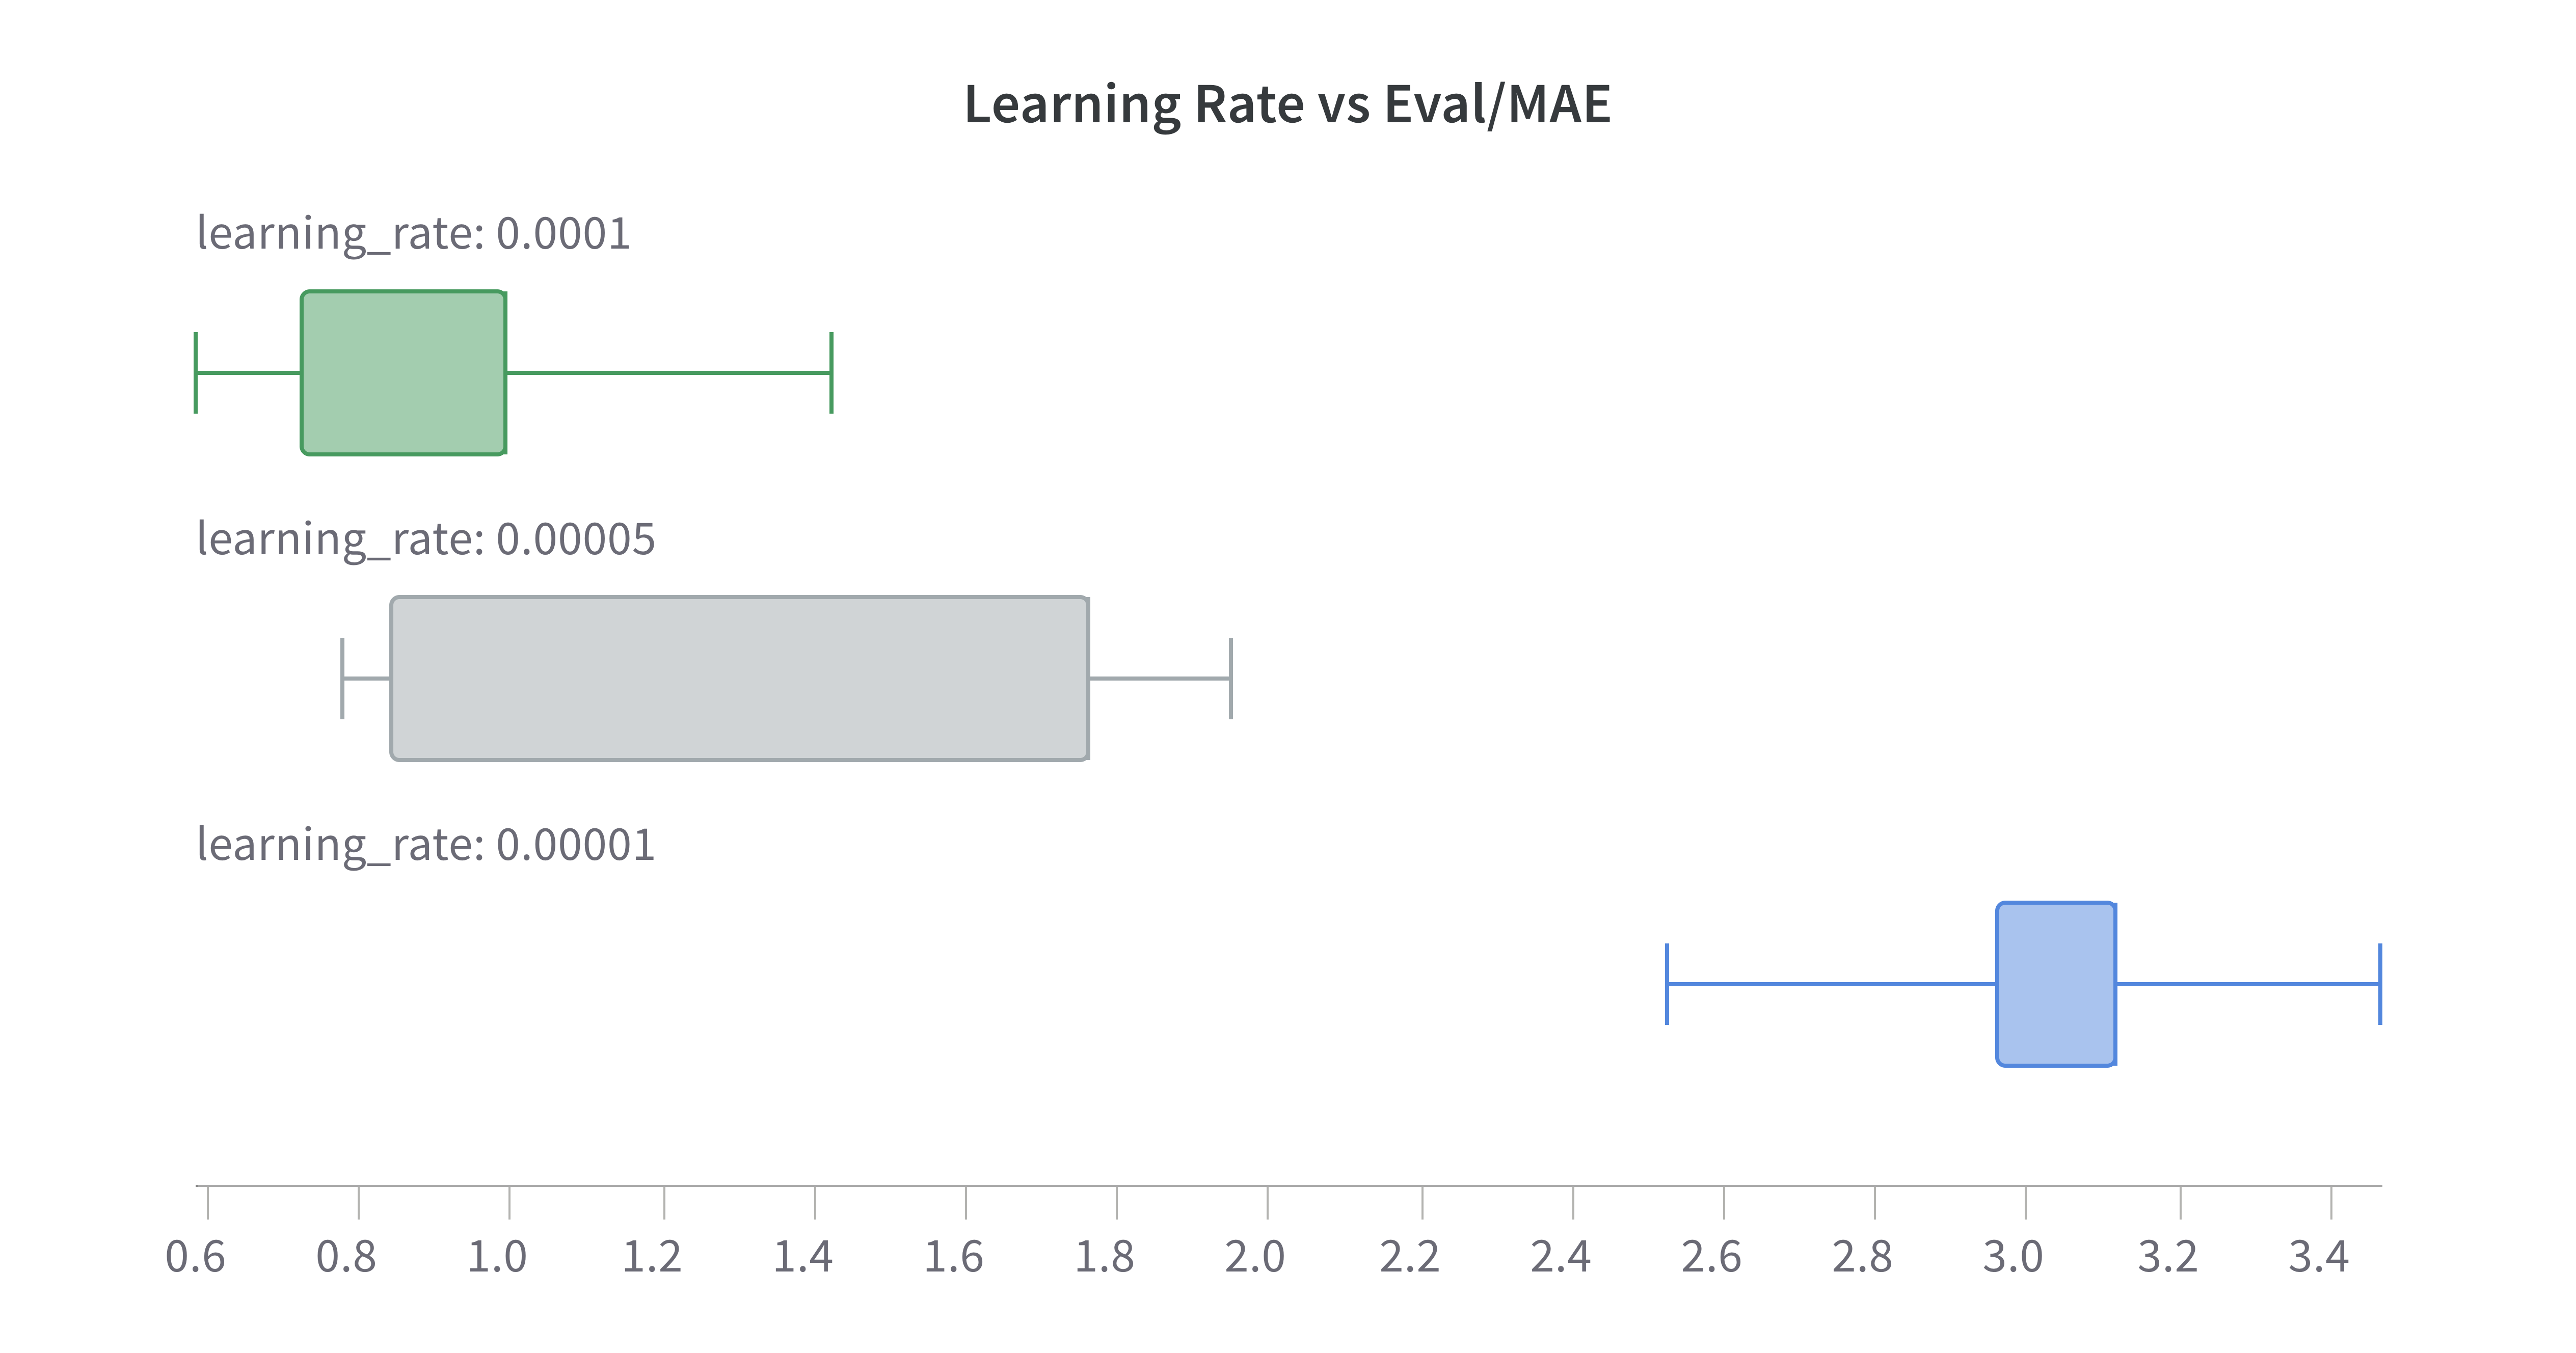
\includegraphics[width=0.48\textwidth]{learningrate}
    \caption{\textbf{Effect of Learning Rate on Model Performance}. Validation MAE for different learning rates (1e-5, 5e-5, 1e-4) showing better results with higher learning rates.}
    \label{fig:hp_learningrate}
\end{figure}
Several clear trends emerged from our analysis:
\begin{itemize}
    \item Learning Rate Impact: Higher learning rates (1e-4) consistently outperformed lower values across all rank and precision combinations, suggesting that more aggressive optimization was beneficial for this task.
    \item Rank Sensitivity: The choice of LoRA rank had a significant impact on performance, with rank 8 yielding the best results across most configurations. Lower ranks (2 and 4) generally resulted in higher MAE values, indicating that the model required more capacity to capture the dynamics of the Lotka-Volterra system.
    \item Precision Trade-offs: The choice of precision (2 vs 3 decimal places) had a noticeable effect on MAE, with 2 decimal places generally leading to lower errors. 
\end{itemize}


\subsubsection*{Optimal Configuration Selection}
Based on our analysis, we selected the following configuration as the best-performing setup for further evaluation:
\begin{itemize}
    \item Learning rate: 1e-4
    \item LoRA rank: 8
    \item Precision: 2 decimal places
    \item LoRA dropout: 0.05
    \item LoRA $\alpha$: 16
\end{itemize}
\subsection*{Context Length Exploration}
After identifying the optimal hyperparameter configuration, we investigated how the length of historical context affects forecasting accuracy. Context length in time series forecasting represents a fundamental trade-off: longer contexts provide more historical patterns for the model to learn from but consume more computational resources and tokens.
\subsubsection*{Experimental Configuration}
We conducted experiments in the same hyperparameter settings as the optimal configuration identified in the previous section.
\begin{itemize}
    \item Shortest context: 128 tokens ($\approx$ 12-13 timesteps)
    \item Medium context: 512 tokens ($\approx$ 50 timesteps)
    \item longest context: 768 tokens ($\approx$ 75 timesteps)
\end{itemize}
For each configuration, we trained models with identical hyperparameters, maintaining consistency in all aspects except the input context length. We evaluated each model on forecasting accuracy for 3 timesteps among 30 sample!! check ahead using our standard test set.

\subsubsection*{Results and Analysis}
Our experiments revealed a clear relationship between context length and forecasting performance:
\begin{figure} [H]
    \centering
    \begin{minipage}{0.48\textwidth}
        \centering
        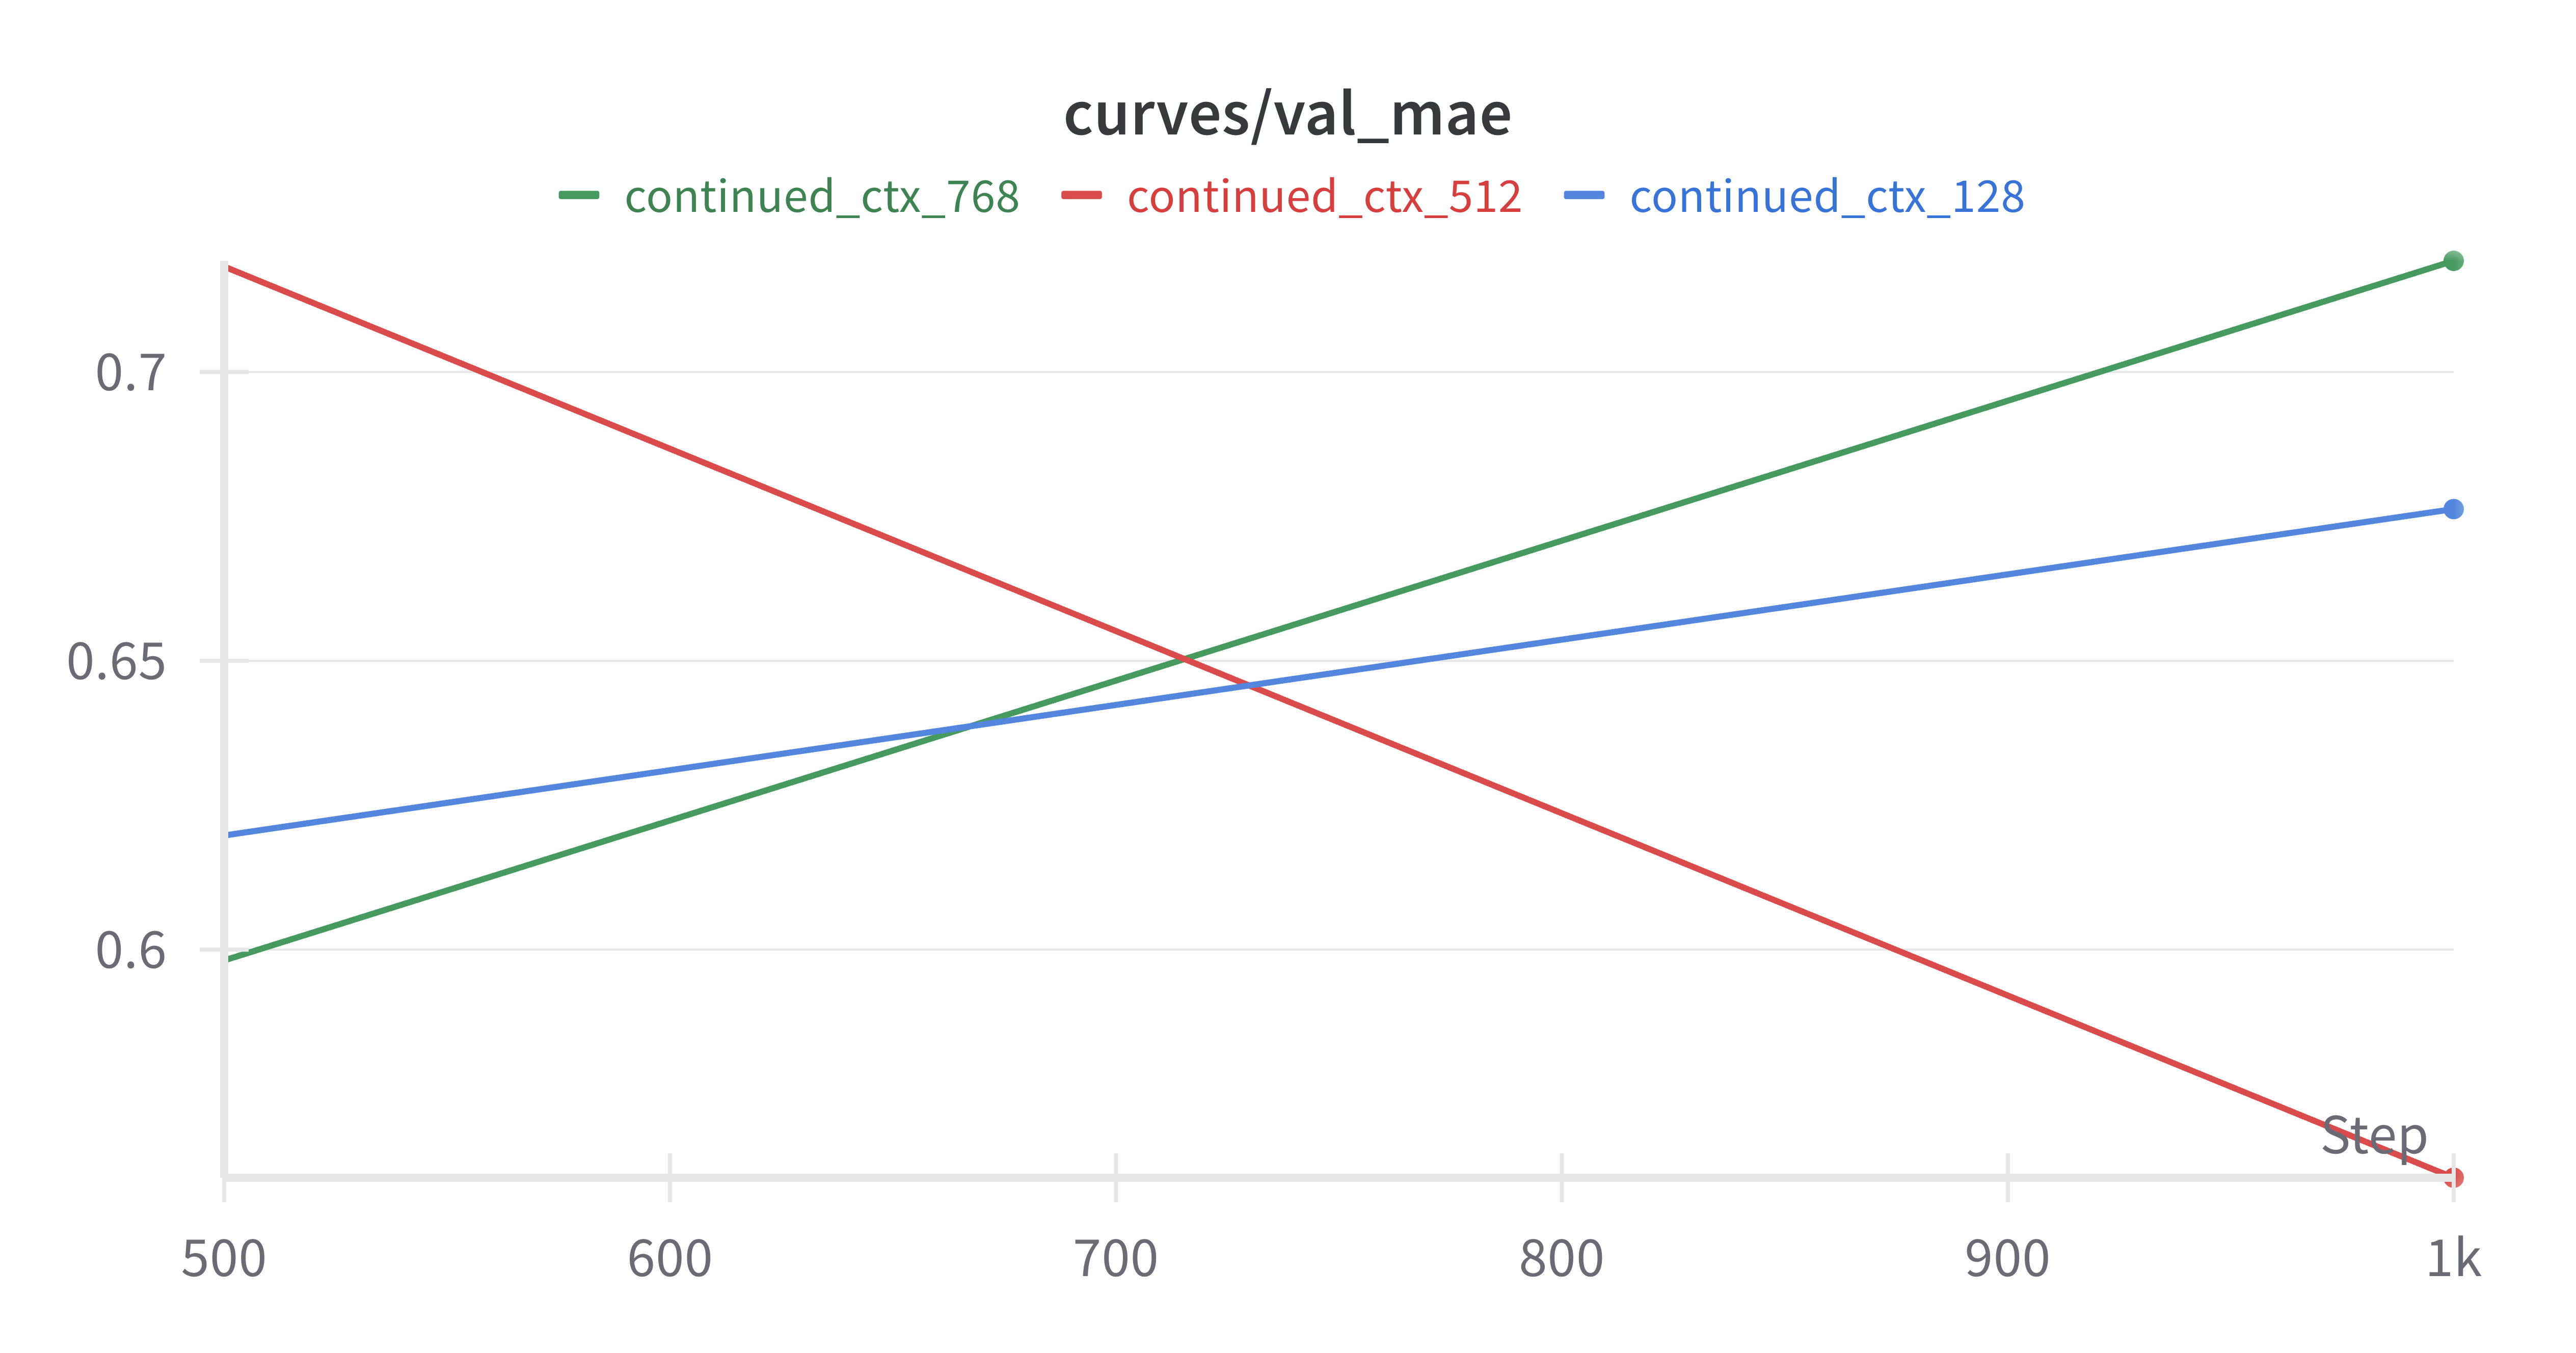
\includegraphics[width=\textwidth]{context_length}
    \end{minipage}
    \caption{\textbf{Context Length Exploration}. Best Validation MAE for different context lengths.}
    \label{fig:context_length}
\end{figure}

The key findings from our context length exploration:
\begin{itemize}
    \item Significant improvement from short to medium context: Increasing from 128 tokens to 512 tokens reduced MAE, indicating that additional historical data substantially improves forecasting accuracy.
    \item Diminishing returns for longer contexts: Further extending context from 512 to 768 tokens increased MAE slightly, suggesting that the model may have reached a saturation point where additional context does not provide significant benefits.
\end{itemize}
\subsubsection*{Periodicity Analysis}
A particularly interesting finding relates to the natural periodicity of the Lotka-Volterra system. Our earlier data analysis revealed average oscillation periods of approximately 20-25 timesteps. The substantial performance improvement when moving from 128 tokens (12-13 timesteps) to 512 tokens (50 timesteps) suggests that providing the model with at least two complete oscillation cycles significantly enhances forecasting accuracy.

This indicates that the model benefits from seeing complete cycles in the input context, allowing it to better learn the phase relationships and amplitude characteristics of the predator-prey dynamics. The modest reduction from extending to 768 tokens (75 timesteps) suggests that the model may have already captured the essential periodicity information within the 512-token context, leading to diminishing returns for longer sequences.


\section*{Model Performance Comparison}

We evaluated three key model configurations on our test set of 150 trajectories: base Qwen2.5 with 2-decimal precision (Base-P2), base Qwen2.5 with 3-decimal precision (Base-P3), and our LoRA-fine-tuned model with 2-decimal precision (LoRA-P2).


\begin{table}[H]
\centering
\begin{tabular}{lccc}
\hline
\textbf{Model} & \textbf{MAE} & \textbf{MSE} & \textbf{Success Rate}  \\
\hline
Base-P2 & 357.2 & 45244228.29 & 100\%  \\
Base-P3 & 3805.9 & 25882364336.72 & 100\% \\
LoRA-P2 & \textbf{0.9742} & \textbf{2.7430} & \textbf{100\%} \\
\hline
\end{tabular}
\caption{Performance comparison across models. MAE/MSE are averaged across all predicted timesteps. Prediction length indicates average number of valid timesteps generated before numerical errors.}
\label{tab:model_comparison}
\end{table}

As shown in Table \ref{tab:model_comparison}, our LoRA-fine-tuned model dramatically outperforms both base models, reducing MAE by over 99.7\%. The base models produce predictions with large, often exponentially growing errors that render them impractical for accurate forecasting, despite generating syntactically valid outputs.

\begin{figure}[H]
    \centering
    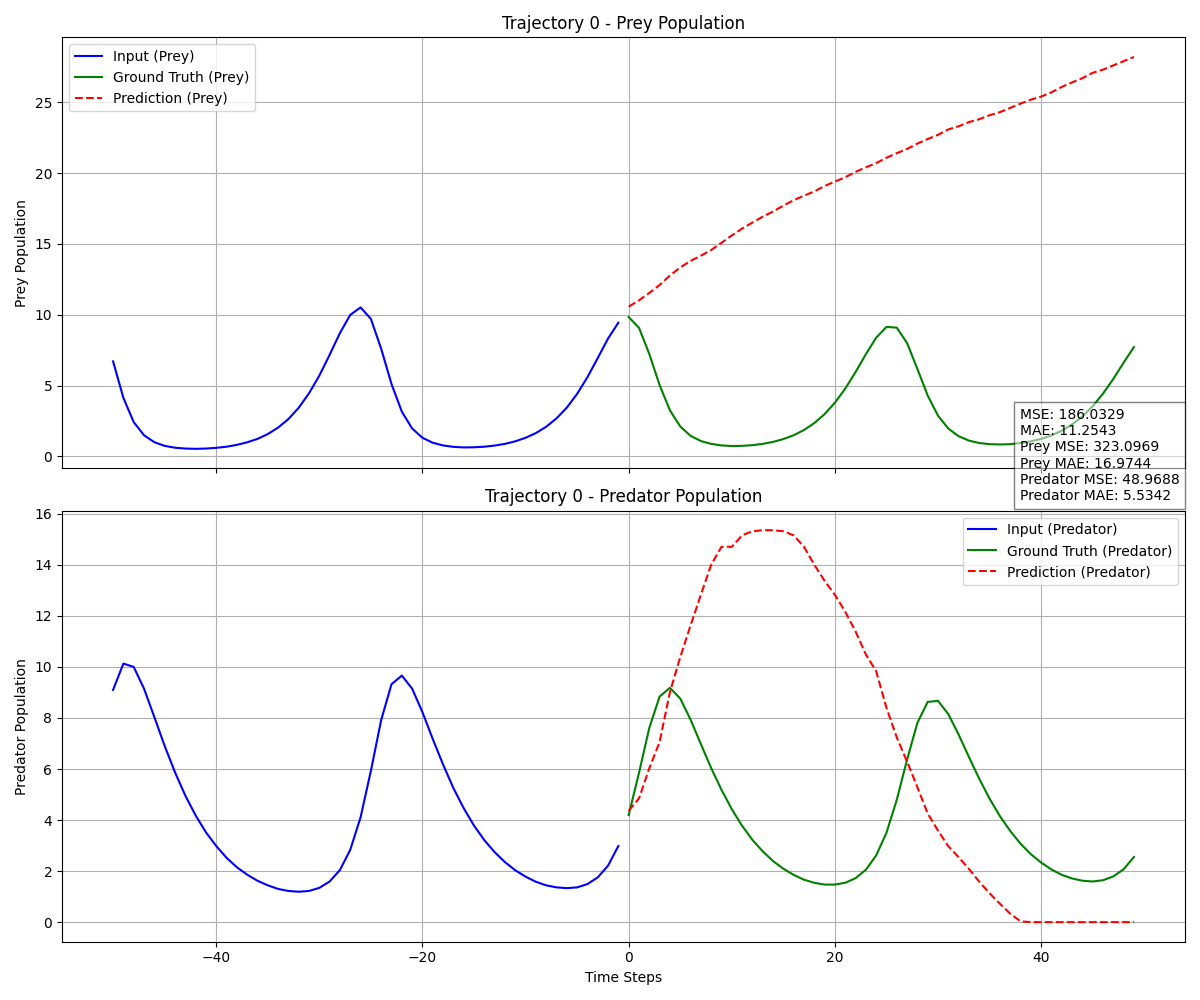
\includegraphics[width=0.6\textwidth]{trajectory_0_prediction_p2}
    \caption{\textbf{Base-P2 Model Predictions}. Base model with 2-decimal precision showing input data (blue), ground truth (green), and model predictions (red) for prey and predator populations.}
    \label{fig:base_p2_predictions_sample}
\end{figure}

\begin{figure}[H]
    \centering
    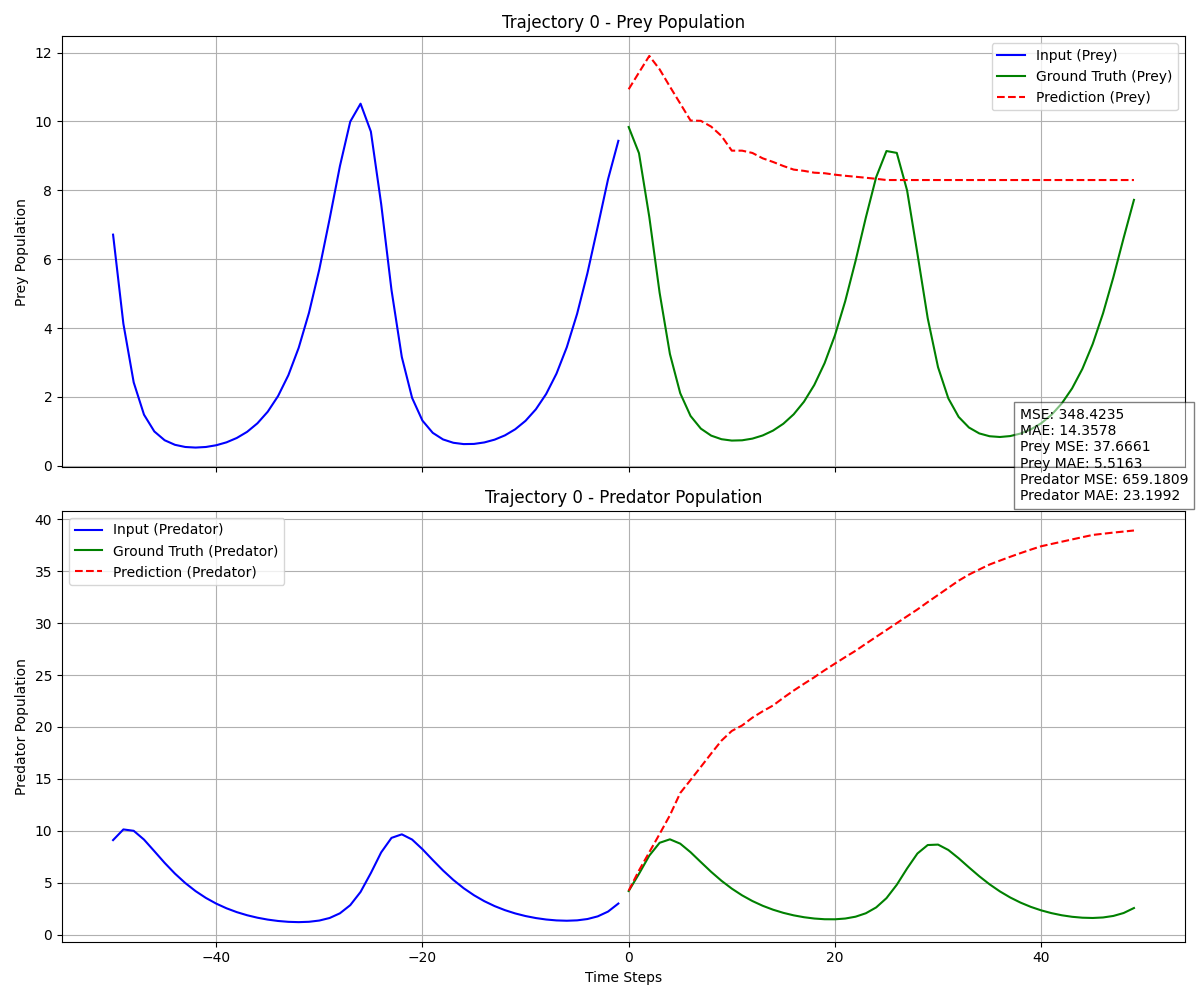
\includegraphics[width=0.6\textwidth]{trajectory_0_prediction_p3}
    \caption{\textbf{Base-P3 Model Predictions}. Base model with 3-decimal precision showing input data (blue), ground truth (green), and model predictions (red) for prey and predator populations.}
    \label{fig:base_p3_predictions_sample}
\end{figure}

\begin{figure}[H]
    \centering
    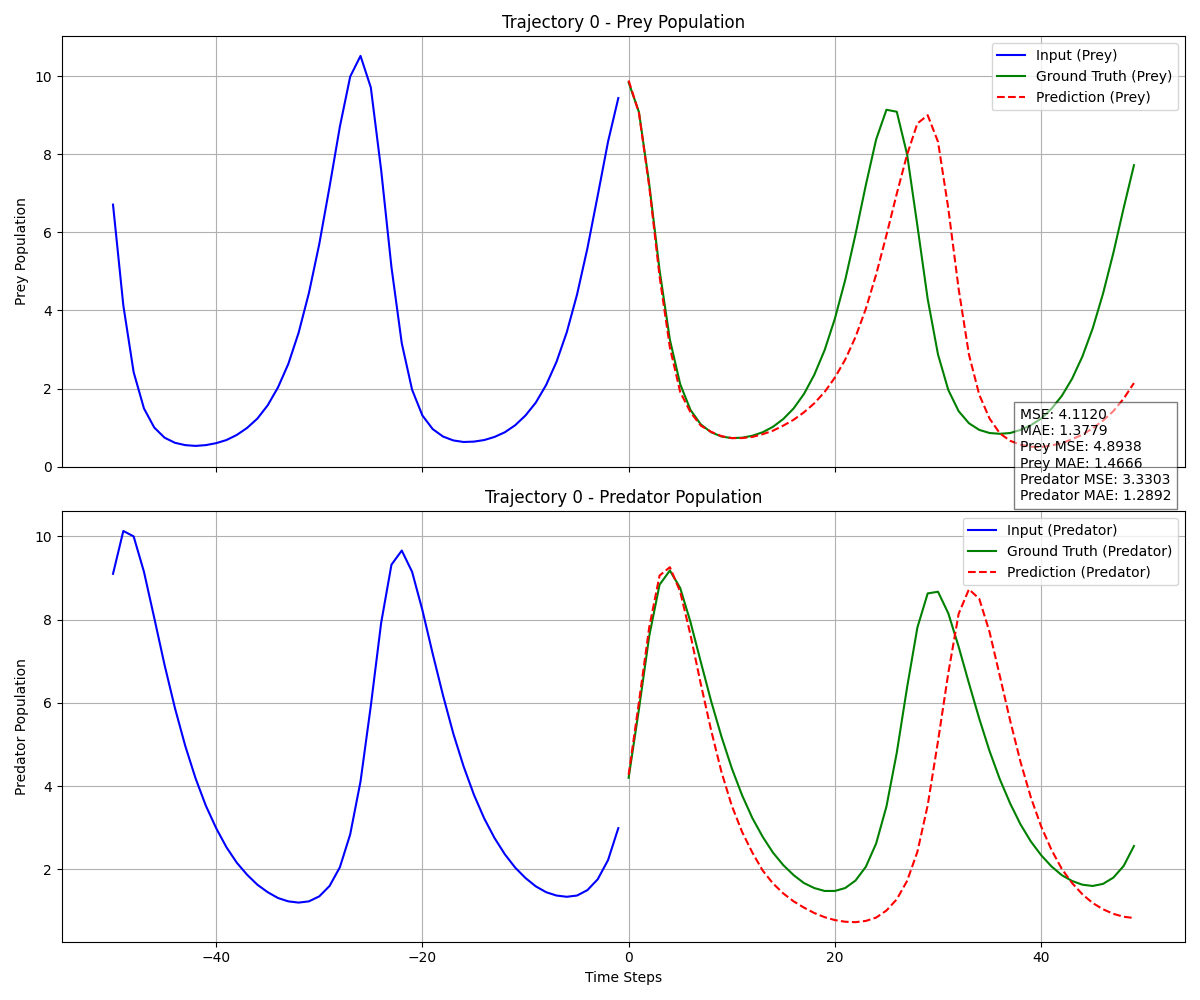
\includegraphics[width=0.6\textwidth]{trajectory_0_prediction_final}
    \caption{\textbf{LoRA-P2 Model Predictions}. Fine-tuned model with 2-decimal precision showing input data (blue), ground truth (green), and model predictions (red) for prey and predator populations.}
    \label{fig:lora_p2_predictions_sample}
\end{figure}

Figures \ref{fig:base_p2_predictions_sample}, \ref{fig:base_p3_predictions_sample}, and \ref{fig:lora_p2_predictions_sample} visualize prediction trajectories for each model. While base models quickly diverge from ground truth values, the LoRA-P2 model closely tracks both prey and predator population cycles, preserving both amplitude and phase relationships. 

\begin{figure}[H]
    \centering
    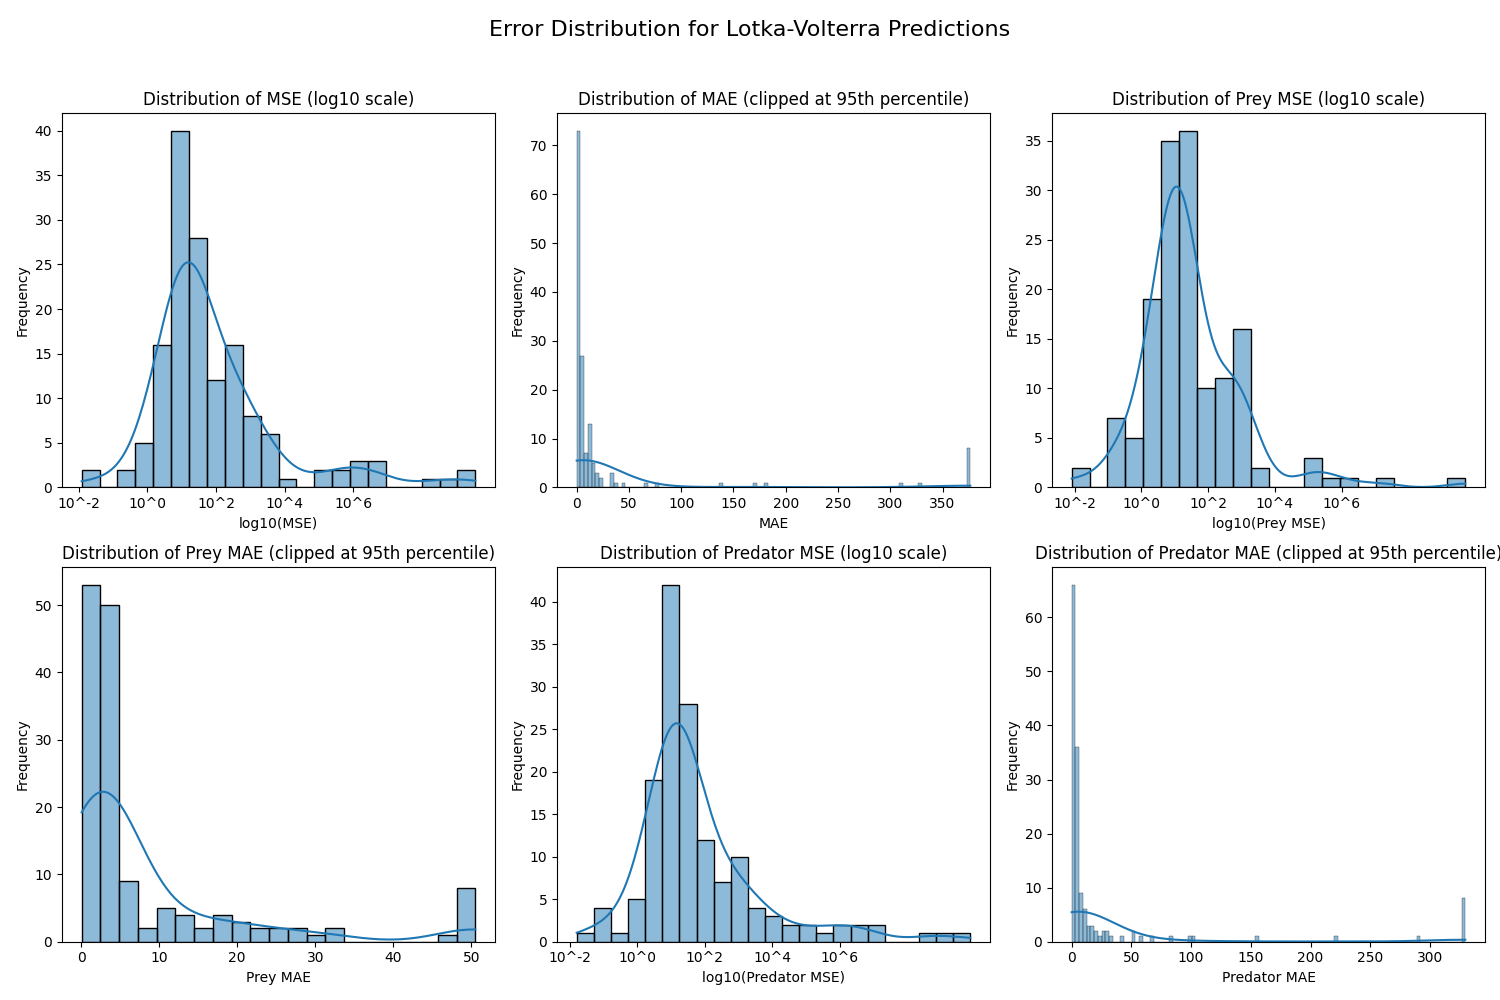
\includegraphics[width=0.8\textwidth]{error_distributions_p2}
    \caption{\textbf{Base-P2 Error Distribution}. Error patterns for the base model with 2-decimal precision across the test dataset.}
    \label{fig:error_p2}
\end{figure}

\begin{figure}[H]
    \centering
    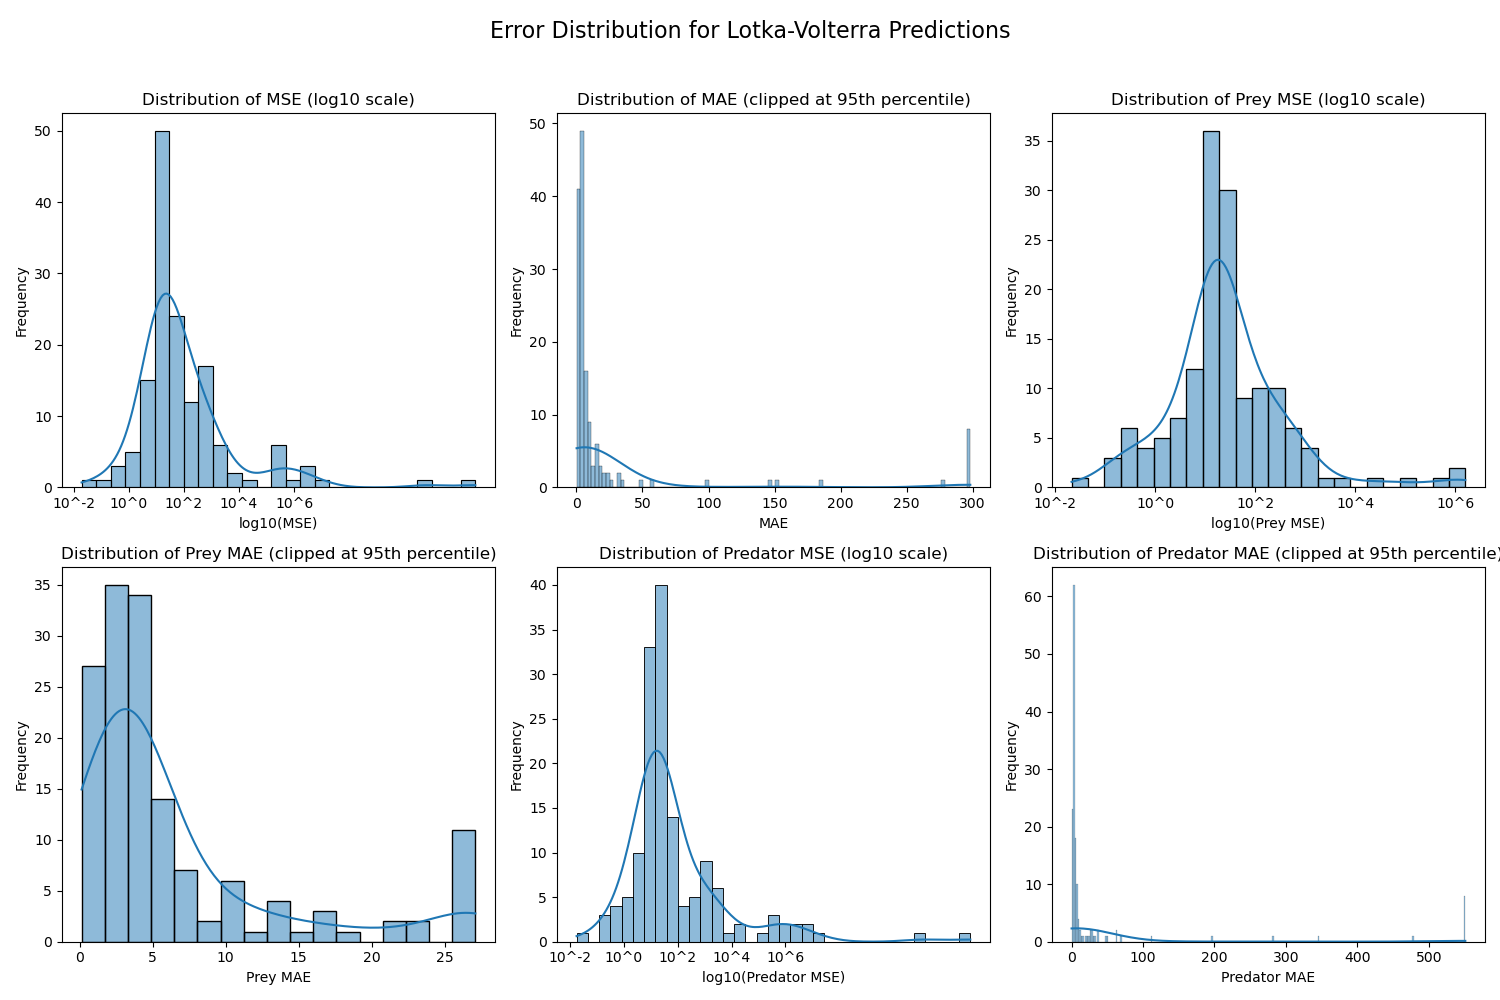
\includegraphics[width=0.8\textwidth]{error_distributions_p3}
    \caption{\textbf{Base-P3 Error Distribution}. Error patterns for the base model with 3-decimal precision across the test dataset.}
    \label{fig:error_p3}
\end{figure}

\begin{figure}[H]
    \centering
    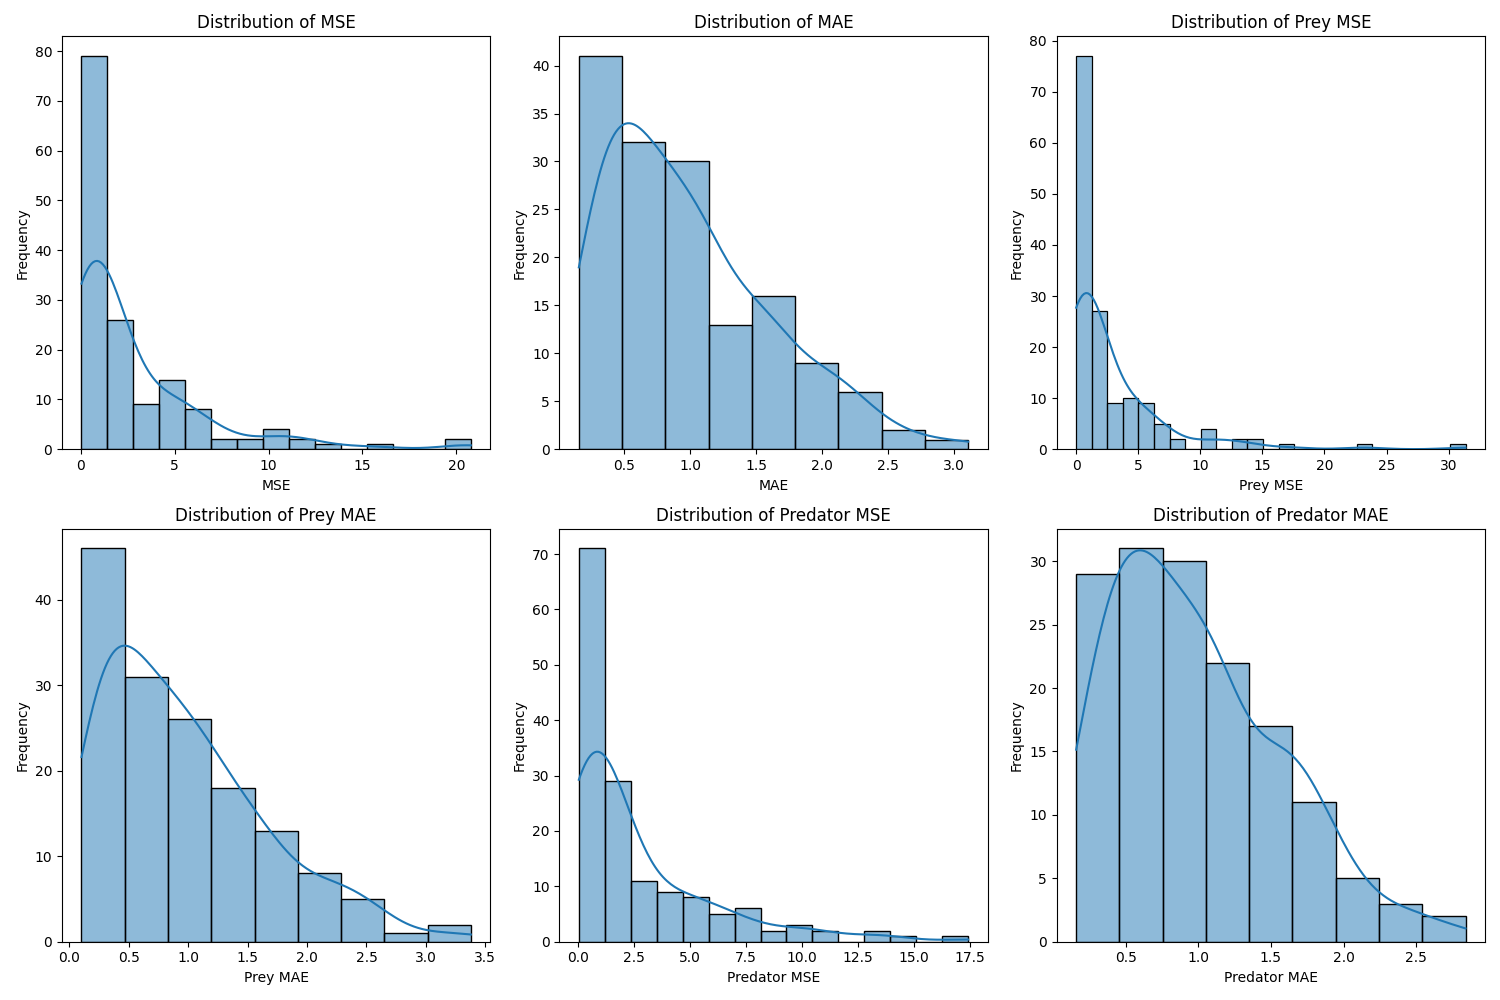
\includegraphics[width=0.8\textwidth]{error_distributions_final}
    \caption{\textbf{LoRA-P2 Error Distribution}. Error patterns for the fine-tuned model with 2-decimal precision across the test dataset.}
    \label{fig:error_lora_p2}
\end{figure}

Error distribution analysis (Figures \ref{fig:error_p2}, \ref{fig:error_p3}, \ref{fig:error_lora_p2}) reveals distinct patterns across models. Base models show rapidly escalating errors with increasing forecast horizon, with error magnitudes often growing exponentially. In contrast, the LoRA model maintains consistently low error rates throughout the prediction window, with only modest increases over time. Notably, the 3-decimal precision format (Base-P3) performs worse than 2-decimal precision (Base-P2).

Figure \ref{fig:error_lora_p2_trajectory} and Figure \ref{fig:error_lora_p3_trajectory} reveal that the 3-decimal precision model experiences even more extreme error values than the Base-P2 model, with some predator prediction errors reaching as high as $10^{13}$ (far right). The model shows similar performance to Base-P2 for easier trajectories but demonstrates catastrophic failure on challenging cases, particularly for predator population predictions. The higher precision appears to make accurate forecasting more difficult for the base model, likely due to increased tokenization complexity.

Figure \ref{fig:error_final_p2_trajectory} reveals several important patterns: 1) approximately one-third of trajectories show very low error (negative log10(MSE) values), indicating MSE values below 1.0; 2) errors gradually increase across trajectories, with the rightmost trajectories showing significantly higher errors (log10(MSE) $>$ 1.0); and 3) prey and predator prediction errors generally follow similar patterns within each trajectory, though prey predictions (blue) tend to have slightly higher errors in the most challenging cases.


\begin{figure} [H]
    \centering
    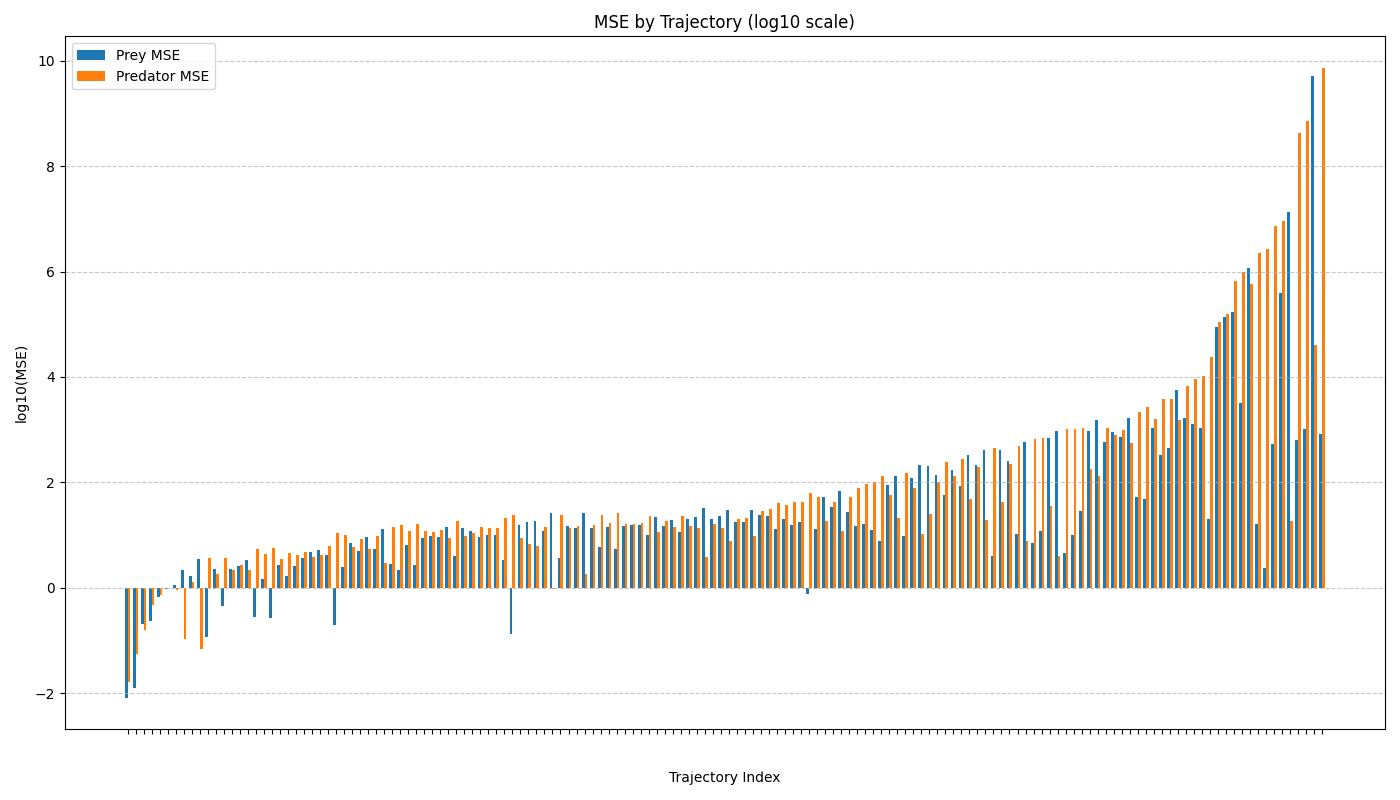
\includegraphics[width=0.8\textwidth]{trajectory_errors_p2}
    \caption{\textbf{MSE by Trajectory (log10 scale) for Base-P2 Model}. This figure presents a detailed analysis of prediction errors across all test trajectories (150 samples), with errors shown on a logarithmic scale (log10). Blue bars represent Mean Squared Error (MSE) for prey population predictions, while orange bars represent MSE for predator population predictions. Trajectories are sorted by increasing maximum error of either population.}
    \label{fig:error_lora_p2_trajectory}
\end{figure}

\begin{figure} [H]
    \centering
    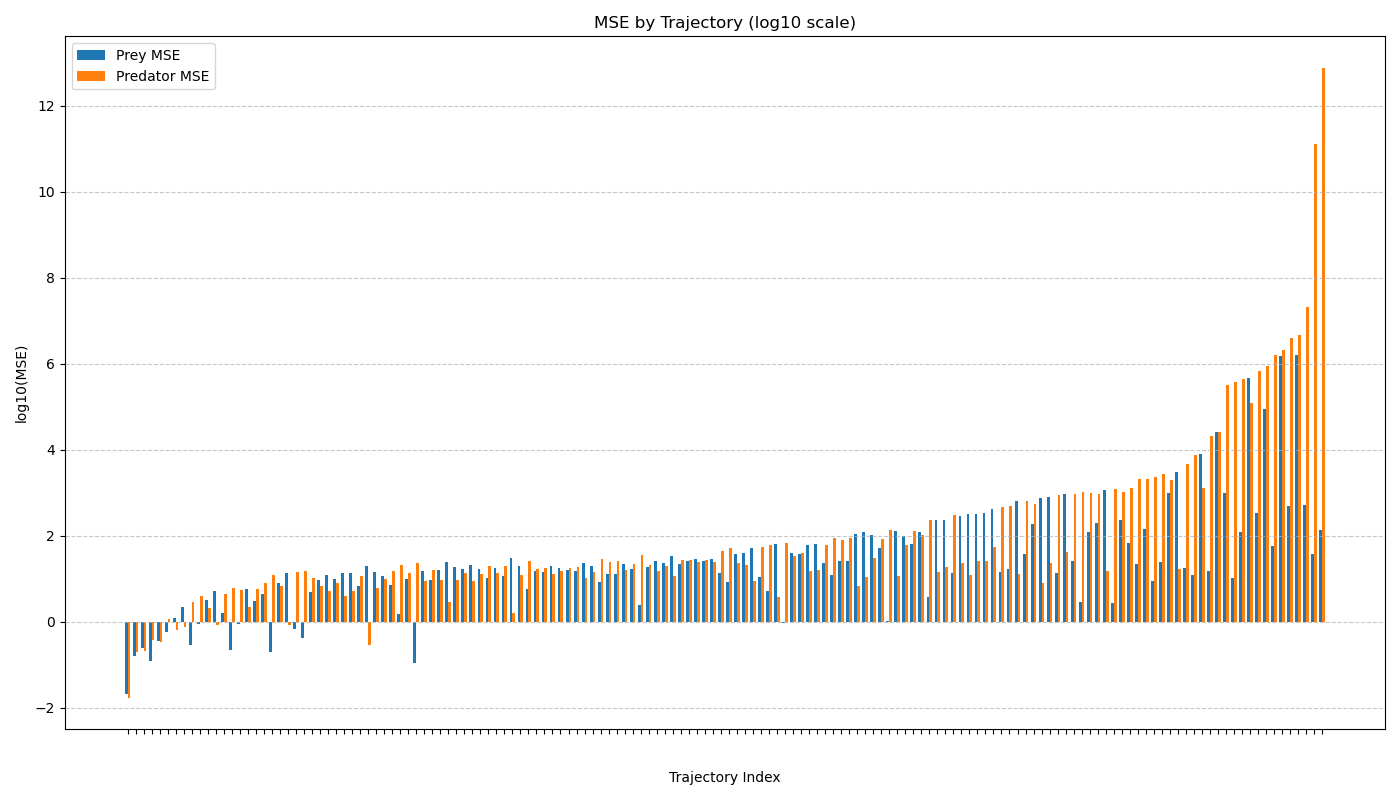
\includegraphics[width=0.8\textwidth]{trajectory_errors_p3}
    \caption{\textbf{MSE by Trajectory (log10 scale) for Base-P3 Model}. This figure presents a detailed analysis of prediction errors across all test trajectories (150 samples), with errors shown on a logarithmic scale (log10). Blue bars represent Mean Squared Error (MSE) for prey population predictions, while orange bars represent MSE for predator population predictions. Trajectories are sorted by increasing maximum error of either population.}
    \label{fig:error_lora_p3_trajectory}
\end{figure}

\begin{figure}[H]
    \centering
    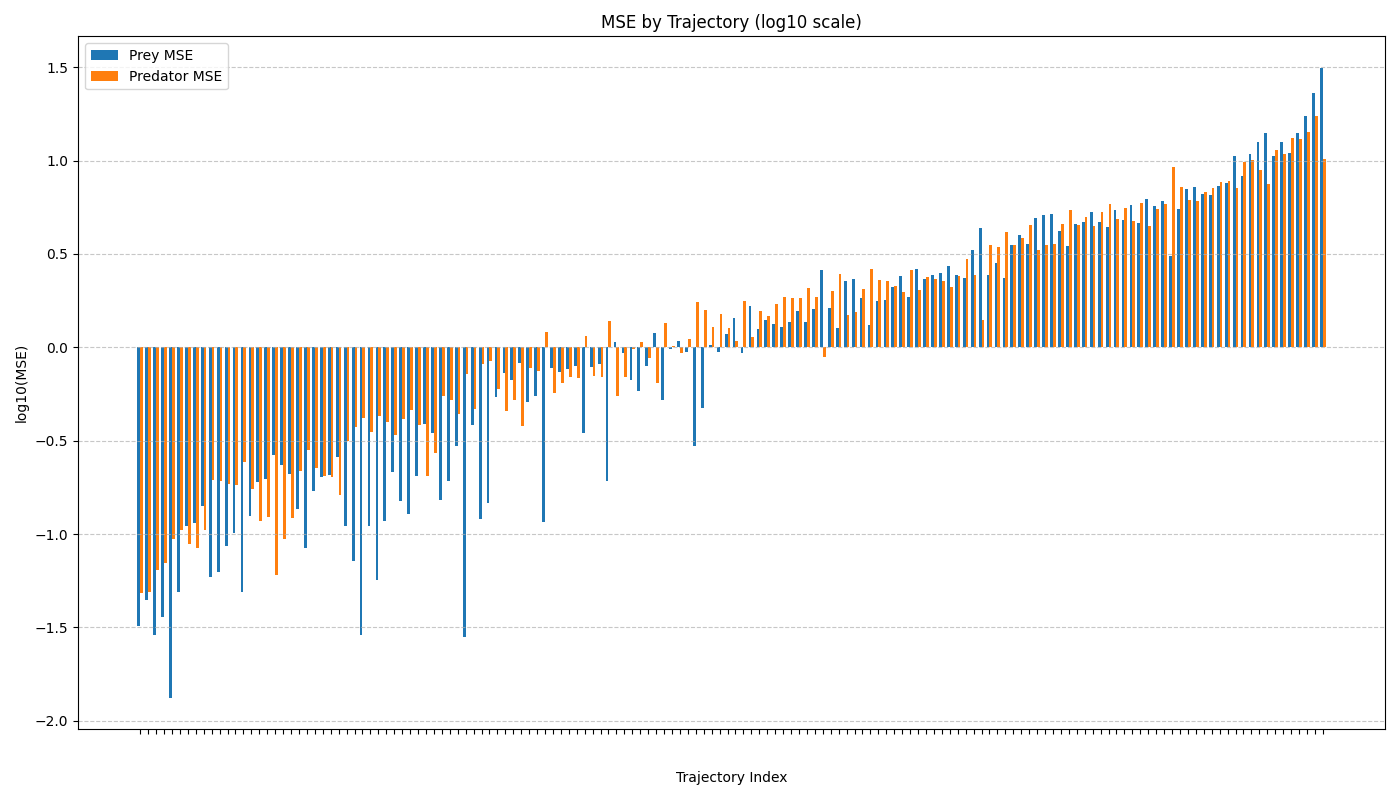
\includegraphics[width=0.8\textwidth]{trajectory_errors}
    \caption{\textbf{MSE by Trajectory (log10 scale) for Final-Lora Model}. This figure presents a detailed analysis of prediction errors across all test trajectories (150 samples), with errors shown on a logarithmic scale (log10). Blue bars represent Mean Squared Error (MSE) for prey population predictions, while orange bars represent MSE for predator population predictions. Trajectories are sorted by increasing maximum error of either population.}
    \label{fig:error_final_p2_trajectory}
\end{figure}

\section*{Discussion}
\subsection*{Theoretical Implications}
Our results reveal a surprising capability of LLMs to model complex dynamical systems through minimal parameter modifications. The successful adaptation to Lotka-Volterra dynamics suggests that transformer architectures inherently capture temporal dependencies and state transitions applicable beyond language. The attention mechanisms appear to effectively model oscillatory behaviors and phase relationships without architectural changes, indicating potential universality in sequence processing across domains. This raises intriguing questions about the fundamental similarities between language modeling and physical system dynamics that warrant further exploration.

\subsection*{Limitations and Future Directions}
Despite promising results, several limitations remain. Our implementation focuses on a relatively simple dynamical system, and generalizability to more complex ecological networks with multiple species or spatial heterogeneity requires investigation. The model's extrapolation capabilities to new parameter regimes—critical for forecasting extreme ecological events—remain untested. Future work should explore hybrid approaches combining LLM flexibility with mechanistic model interpretability, and extend these methods to handle irregular sampling, missing data, and observational noise typical in ecological time series.
\section*{Appendix}
\subsection*{Detailed FLOP Calculation}

This section provides a comprehensive accounting of the floating-point operations (FLOPs) used in our experiments with the Qwen2.5-0.5B model, based on our custom FLOP tracking implementation.

\subsubsection*{Forward Pass Components}

For a single forward pass with sequence length $S$, batch size $B$, hidden dimension $H=896$, intermediate dimension $I=4864$, and vocabulary size $V=151,936$, we calculate FLOPs for each component as follows:

\paragraph{Embedding Layer}
The token embedding lookup is primarily a memory operation rather than computational, counted as:
\begin{equation}
\text{FLOPs}_{\text{embedding}} = B \times S \times H = 64 \times 512 \times 896 \approx 2.94 \times 10^7 \text{ FLOPs}
\end{equation}

\paragraph{Attention Mechanism with LoRA}
For each attention layer:
\begin{enumerate}
    \item \textbf{Query projection with LoRA}: For modules with LoRA enabled (rank $r=8$):
    \begin{align}
    \text{FLOPs}_{\text{q\_proj}} &= \text{FLOPs}_{\text{original}} + \text{FLOPs}_{x \times A^T} + \text{FLOPs}_{(xA^T) \times B^T}\\
    &= B\times S \times H \times (2H-1) \\
    &+ B\times S \times r \times (2H-1) + B\times S \times H \times (2r-1)
    \end{align}
    
    \item \textbf{Key/Value projections}: Similar to query.
    \item \textbf{RoPE}: $B\times S \times 3 \times \text{num\_heads} \times \text{head\_dim} + 0.5 \times B \times S \times \text{num\_heads} \times \text{head\_dim}$, here we only negate half of the original length of x.
    \item \textbf{Attention scores}: $B\times S \times \text{num\_heads} \times S \times (2 \times \text{head\_dim} - 1)$
    \item \textbf{Attention mask}: $B \times \text{num\_heads} \times S \times S$
    \item \textbf{Attention softmax}: $B \times \text{num\_heads} \times S \times (12S - 1)$
    \item \textbf{Weighted sum}: $B \times \text{num\_heads} \times S \times \text{head\_dim} \times (2S - 1)$
    \item \textbf{Output projection}: Similar structure to query projection if LoRA is applied
\end{enumerate}

\paragraph{Feed-Forward Network}
\begin{enumerate}
    \item \textbf{Gate and Up projections}: $2 \times B\times S \times I \times (2H - 1)$
    \item \textbf{SwiGLU activation}: $B\times S \times I \times 14$
    \item \textbf{Element-wise multiplication}: $B\times S \times I$
    \item \textbf{Down projection}: $B\times S \times H \times (2I - 1)$
\end{enumerate}

\paragraph{Layer Normalization and Residuals}
\begin{enumerate}
    \item \textbf{RMSNorm (2 per layer)}: $2 \times B\times S \times (4H + 12)$
    \item \textbf{Residual connections}: $2 \times B\times S \times H$
\end{enumerate}

\paragraph{Output Layer}
\begin{enumerate}
    \item \textbf{Final RMSNorm}: $ B \times S (4 \times H+12) FLOPs$
    \item \textbf{LM head}: $2 \times B \times S \times H \times V = 2 \times B \times S \times 896 \times 151936$ FLOPs
\end{enumerate}

\subsubsection*{Total Forward Pass FLOPs}

For our configuration with $H=896$, $I=4864$, and 24 layers, the total forward pass FLOPs for batch size $B=4$ and sequence length $S=512$ is approximately:
\begin{align}
\text{FLOPs}_{\text{forward}} \approx & 1.98 \times 10^{12} \text{ FLOPs} 
\end{align}

\subsubsection*{Training Step FLOPs}

For training, our implementation uses the standard approximation that backward pass requires twice the computation of the forward pass (in the same setting as in forward pass):
\begin{equation}
\text{FLOPs}_{\text{training\_step}} = \text{FLOPs}_{\text{forward}} + 2 \times \text{FLOPs}_{\text{forward}} \approx 5.94 \times 10^{12} \text{ FLOPs}
\end{equation}

\subsubsection*{Budget Allocation and Usage}

Our implementation tracked FLOPs throughout the experimental process, including:
\begin{table}[H]
    \centering
    \begin{tabular}{lcc}
    \hline
    \textbf{Experiment} & \textbf{Total FLOPs} & \textbf{Budget Percentage} \\
    \hline
    \multicolumn{3}{c}{\textbf{Hyperparameter Grid Search (18 configurations)}} \\
    \hline
    Average per Hyperparameter Config & 2.70$\times$ 10$^{15}$ & 2.7\% \\
    Total Grid Search (18 Experiments) & 4.86 $\times$ 10$^{16}$ & 48.6\% \\
    \hline
    \multicolumn{3}{c}{\textbf{Context Length Evaluation}} \\
    \hline
    Context Length 768 & 9.10 $\times$ 10$^{15}$ & 9.1\% \\
    Context Length 512 & 5.94$\times$ 10$^{15}$ & 5.9\% \\
    Context Length 128 & 1.43 $\times$ 10$^{15}$ & 1.4\% \\
    \hline
    \multicolumn{3}{c}{\textbf{Final Fine-tuning (LoRA)}} \\
    \hline
    LoRA (r=8, $\alpha$=16, lr=1e-04, bs=4) & 3.50 $\times$ 10$^{16}$ & 35\% \\
    \hline
    \multicolumn{3}{c}{\textbf{Overall FLOP Usage}} \\
    \hline
    Total Experimental FLOPs & 1.0 $\times$ 10$^{17}$ & 100.0\% \\
    Maximum Budget & 1.0 $\times$ 10$^{17}$ & 100.0\% \\
    \hline
    \end{tabular}
    \caption{FLOPs Usage Across Experiments}
    \label{tab:flops_usage}
    \end{table}
    

\bibliographystyle{plain}
\bibliography{references}
\end{document}